\PassOptionsToPackage{sort&compress}{natbib}
\documentclass[oneside]{fast-nuces-bs}

\usepackage{mathptmx}% Times Roman font
\usepackage[T1]{fontenc}
\usepackage{sectsty}
\usepackage{tikz-uml}
\usepackage{titlesec}

% ---- added for the CARAZONE report body -------------------------------------
% These are required by the diagrams and tables in the chapters. The class
% already loads tikz, graphicx, amsmath and amssymb.
\usetikzlibrary{positioning,arrows.meta,shapes.geometric,fit,calc}
\usepackage{booktabs}
\usepackage{longtable}
\usepackage{array}
\usepackage{float}
\graphicspath{{figures/}{ThesisFigs/}{./}}
% The class's \maketitle ends the title page with \null\vfill. The title page
% is already full, so that overflows into a blank page carrying a stray page
% number. This removes it without modifying fast-nuces-bs.cls, so the stock
% class file can still be submitted unchanged. If the patch ever fails to
% apply, the build still succeeds and the blank page simply returns.
\patchcmd{\maketitle}{\null\vfill}{}{}{}
% The class loads natbib in author-year mode, but IEEEtran.bst is a numeric
% style. Without this line the two disagree and natbib raises an error.
% This switches citations to numeric and leaves the class file untouched.
\setcitestyle{numbers,square,comma}
% -----------------------------------------------------------------------------

% Information about the Thesis
% -----------------------------------------------------------------------------
% (All are compulsory, do not delete any line other than author Information)
% This project has two members, so \authorthree and \authorfour are omitted.
%%%%%%%%%%%%%%%%%%%%%%%%%%%%%%%%%%%%%%%%%%%%%%%%%%%%%%%%%%%%%%%%%%%%%%%%%%%%%%%
\department{FAST School of Computing}
\faculty{Computer Science}
\degreeyear{2026}
\degreemonth{October}
\degreename{Computer Science}
\campuscity{Islamabad}
\authorone{Adeena Zaib}{23I-0674}
\authortwo{Khaula Bilqees}{23I-0574}
\supervisor{Dr. Muhammad Rizwan}
\sessionduration{2023-2027}
\cosupervisor{Dr. Hina Ayaz}
% The class defines \deanname, \directorname, \hodname and
% \fypcoordinatorname, but no page in this template prints them, so they are
% omitted. Restore them if your department adds a signature page.
\title{CARAZONE: Federated Intrusion Detection for Timing Attacks
       in Automotive Zonal TSN Architectures}
%%%%%%%%%%%%%%%%%%%%%%%%%%%%%%%%%%%%%%%%%%%%%%%%%%%%%%%%%%%%%%%%%%%%%%%%%%%%%%%

% The template's front-matter files reference these; defined here so they
% resolve to the same values as the metadata above.
\newcommand{\projecttitle}{\@title}
\newcommand{\studentone}{Adeena Zaib}
\newcommand{\studenttwo}{Khaula Bilqees}

%%%%%%%%%%%%%%%%%%%%%%%%%%%%%%%%%%%%%%%%%%%%%%%%%%%%%%%%%%%%%%%%%%%%%%%%%%%%%%
% Former document starts below this
\begin{document}

% The class calls \maketitle itself via \AfterEndPreamble, so it must NOT be
% called here: doing so prints the title page twice. The title page already
% ends with a page break, so no \cleardoublepage is needed before the front
% matter; adding one leaves a blank page after the title.
\pagenumbering{roman}
\chapter*{Students' Submission}
\addcontentsline{toc}{chapter}{Students' Submission}
We certify that this report is submitted as the FYP-1 mid-report for the project
titled \emph{CARAZONE: Federated Intrusion Detection for Timing Attacks in
Automotive Zonal TSN Architectures}.

\begin{tabbing}
Student 1: Adeena Zaib \hspace{3cm} \= Signature: \rule{4cm}{0.4pt} \\[2em]
Student 2: Khaula Bilqees \> Signature: \rule{4cm}{0.4pt}
\end{tabbing}

% [[FILL]] roll numbers on the title page

\chapter*{Anti-Plagiarism Statement}
\addcontentsline{toc}{chapter}{Anti-Plagiarism Statement}
The students certify that this report is their own work and that all sources used in preparing the report have been appropriately acknowledged and referenced.

\chapter*{Authors' Declaration}
\addcontentsline{toc}{chapter}{Authors' Declaration}
We declare that the work documented in this report represents the work completed by the project team up to the FYP-1 mid-report stage. Contributions, tools, external components, and relevant sources are disclosed where applicable.

\chapter*{Abstract}
\addcontentsline{toc}{chapter}{Abstract}
Automotive zonal electrical/electronic architectures place safety-critical control
traffic, sensor streams and infotainment on a single Ethernet backbone, and rely on
Time-Sensitive Networking (TSN) to keep that traffic deterministic. Determinism
depends on the generalised Precision Time Protocol (gPTP, IEEE 802.1AS), which was
standardised without security controls. An attacker who manipulates synchronisation
can therefore degrade timing guarantees without altering packet content or traffic
volume, which places the attack outside the detection surface of conventional
content- and volume-based intrusion detection.

This project develops a federated intrusion detection system that operates on
TSN protocol-native signals rather than generic traffic statistics. Zone controllers
act as federated clients, each extracting timing features from locally observed gPTP
state and training a shared model architecture; a central vehicle compute unit
aggregates model parameters without receiving raw feature records.

At the mid-report stage, a four-zone automotive TSN topology has been implemented in
OMNeT++/INET with gPTP synchronisation, and three attack configurations have been
instrumented. Fifteen seeded simulation runs (three benign and twelve delay-attack runs covering
four target zones at three seeds each) have produced 225 recorded vectors,
converted by a Python extraction pipeline into 4{,}740 labelled feature windows.
Delay-attack injection has been validated against the expected theoretical signature.
A cross-zone residual feature has been added and a centralized detector trained,
establishing the project's central premise ahead of schedule: features computed within
a single zone detect the attack no better than a majority-class predictor
(macro-F1 0.48--0.54 against a floor of 0.47), whereas two cross-zone residual features
reach 0.95--0.98 macro-F1 with detection two synchronisation intervals after onset.
Two negative results are reported: oscillator drift manipulation is not realisable as
a runtime attack under the simulation framework, and no fixed threshold, neither a
maximum nor a percentile, separates attack from benign behaviour, because the
synchronisation convergence transient produces residuals 2.7 times larger than the
attack does. Remaining work for FYP-2 comprises zone heterogeneity, the federated
training pipeline, and the comparative evaluation.

\chapter*{Acknowledgments}
\addcontentsline{toc}{chapter}{Acknowledgments}
The project team acknowledges the guidance and support received from the project supervisor, faculty members, and other contributors.

\chapter*{Executive Summary}
\addcontentsline{toc}{chapter}{Executive Summary}
\textbf{Problem.} Zonal automotive architectures converge previously isolated
domains onto one TSN Ethernet backbone. Isolation that was formerly physical is
now logical, enforced by time-aware scheduling that depends on a shared time base
distributed by gPTP. gPTP carries no authentication, and a class of attacks against
it, notably asymmetric delay injection, is not addressed by cryptographic
countermeasures, because delaying an authentic message is as effective as forging
one. The resulting anomalies are invisible to intrusion detection built on payload
inspection or traffic-volume statistics.

\textbf{Gap.} Existing work divides into three groups, none of which covers this
intersection: industrial federated TSN-IDS work that is not automotive or zonal;
automotive IDS work that targets the CAN bus and therefore has no gate schedule or
synchronisation tree to observe; and TSN security research that characterises attack
impact without federated, zone-level operational detection.

\textbf{Approach.} A centralized cross-silo horizontal federated learning design in
which each zone controller is a client. Clients extract windowed timing features from
gPTP state, train a shared compact model locally, and exchange only parameters with
the central vehicle compute unit. The contribution is the use of protocol-native,
schedule-derived signals as the detection feature space, evaluated against a
generic-traffic-feature control arm and against centralized and local-only training
baselines.

\textbf{Status at mid-report.} The simulation environment, attack injection harness
and feature extraction pipeline are complete and reproducible across seeded runs. A
centralized detector has been trained and the feature ablation establishing success
criterion SC-2 has been completed. The federated layer is designed but not yet
implemented. One attack class is validated, one is documented as unrealisable under the
current framework, and one is instrumented but not yet extracted.

\textbf{Principal risk.} All zones currently carry identical traffic profiles, which
would make the federated comparison null by construction; differentiated per-zone
profiles are scheduled first in Iteration~04. A secondary concern is that the injected
attack is large relative to the benign steady-state envelope, so an attack-intensity
sweep is required to establish where detection degrades.

% The class's \maketitle already emits \tableofcontents, \listoffigures and
% \listoftables immediately after the title page. Calling them again here, as
% the stock template does, prints three empty headings on a page of their own.
\chapter*{List of Abbreviations}
\addcontentsline{toc}{chapter}{List of Abbreviations}
\begin{tabbing}
\hspace{2.5cm}\= \kill
AVTP \> Audio Video Transport Protocol \\
BMCA \> Best Master Clock Algorithm \\
CVC  \> Central Vehicle Compute \\
E/E  \> Electrical/Electronic (architecture) \\
FedAvg \> Federated Averaging \\
FL \> Federated Learning \\
FR \> Functional Requirement \\
FRER \> Frame Replication and Elimination for Reliability (IEEE 802.1CB) \\
GCL \> Gate Control List \\
GM \> Grandmaster (clock) \\
gPTP \> generalised Precision Time Protocol (IEEE 802.1AS) \\
HFL \> Horizontal Federated Learning \\
IDS \> Intrusion Detection System \\
MLP \> Multilayer Perceptron \\
NFR \> Non-Functional Requirement \\
TAS \> Time-Aware Shaper (IEEE 802.1Qbv) \\
TSN \> Time-Sensitive Networking \\
TT \> Time-Triggered (traffic class) \\
vSOC \> Vehicle Security Operations Centre \\
ZC \> Zone Controller
\end{tabbing}

% ============================================================


\cleardoublepage
\pagenumbering{arabic}
\chapter{Introduction and Project Vision}
% ============================================================

\section{Project Overview}
CARAZONE is a simulation-based federated intrusion detection system for the
Time-Sensitive Networking (TSN) Ethernet backbone of an automotive zonal
electrical/electronic architecture. The system observes TSN protocol-native signals
at each zone controller, extracts timing features over fixed observation windows,
trains a shared detection model across zones using federated learning without
centralising raw feature records, and emits attributed alerts identifying the attack
class and the affected zone.

The delivered artefact is a laboratory validation and research tool, not a production
vehicle component. It comprises a configurable zonal TSN simulation, an attack
injection harness producing ground-truth labels, a feature extraction pipeline, a
federated training and evaluation workflow, and an alert presentation surface.

\section{Problem Statement}
No existing work federates intrusion detection built on TSN's own protocol-native
signals for automotive zonal Ethernet backbones, a topology with heterogeneous
zone-level data that current federated TSN-IDS work (industrial) and automotive IDS
work (CAN bus) both miss.

Concretely: in a zonal architecture the isolation between safety-critical and
non-critical traffic is enforced logically by time-aware scheduling rather than
physically by separate wiring. That scheduling is meaningful only because every node
agrees on the current time. An adversary who corrupts the shared time base therefore
degrades timing guarantees across the backbone without injecting malformed frames,
without raising traffic volume, and without altering any payload. Detection
approaches that observe payload content or flow statistics have no visibility of
this failure mode.

\section{Problem Context and Motivation}
\label{sec:problem-context}
Automotive E/E architecture is migrating from roughly 70--100 distributed ECUs on
segmented buses toward a small number of zone controllers linked by a high-bandwidth
Ethernet backbone. TSN provides the determinism that the displaced buses supplied
natively. Two TSN mechanisms are central: IEEE~802.1AS (gPTP) distributes a common
time base, and IEEE~802.1Qbv (TAS) uses that time base to gate traffic classes into
scheduled windows.

Neither mechanism was standardised with security controls. For gPTP specifically,
cryptographic authentication does not close the full threat surface: an asymmetric
delay attack manipulates the \emph{timing} of authentic messages, corrupting the
peer-delay computation on which offset correction depends. Authentication confirms
that a message is genuine; it cannot establish that the message arrived when it
should have.

The consequence is not immediate catastrophic failure. End-to-end protection
mechanisms at the application layer detect missed updates and degrade to fail-safe
states. The realistic impact is stealthy availability denial: forced degradation,
limp-home transitions and driver warnings at a time of the attacker's choosing. This
is a detection problem rather than a prevention problem, and it is the problem this
project addresses.

\section{Project Vision}
To demonstrate that intrusion detection for automotive zonal TSN backbones is more
effective when built on protocol-native timing signals than on generic traffic
statistics, and that such detection can be trained across heterogeneous zones using
federated learning without centralising raw per-zone observations.

\section{Project Objectives}
\begin{enumerate}
  \item \textbf{O1.} Implement a configurable multi-zone automotive TSN topology in
        OMNeT++/INET with gPTP synchronisation and reproducible seeded execution.
  \item \textbf{O2.} Implement an attack injection harness for TSN timing attacks that
        produces ground-truth labels with zone, time-window and attack-class attribution.
  \item \textbf{O3.} Implement a passive feature extraction pipeline converting raw
        simulation output into labelled, windowed, protocol-native feature vectors.
  \item \textbf{O4.} Train and evaluate a detection model on those features, and
        demonstrate by controlled comparison whether protocol-native features
        outperform generic traffic features on the same scenarios.
  \item \textbf{O5.} Implement federated training across per-zone clients and compare
        it against centralized-pooled and local-only training baselines.
  \item \textbf{O6.} Produce attributed alerts carrying attack class, affected zone,
        time window and confidence, and present them through an operator-facing surface.
\end{enumerate}

Objectives O1--O3 are complete at the mid-report stage. O4--O6 are scheduled for
Iterations~03 and~04.

\section{Project Scope}
\label{sec:scope}

\subsection*{Scope statement}
The project targets the TSN Ethernet backbone connecting zone controllers to central
compute in automotive zonal E/E architectures, focusing specifically on attacks
against TSN features. The project trains a detection model across simulated
zone/platform clients standing in for heterogeneous vehicle architectures (zonal
topologies), using federated learning. Evaluation compares this federated approach
against a centralized version of the same detector and against existing
non-federated detection work, using synthetic attack datasets generated via a TSN
simulation framework.

\subsection*{Included and excluded functionality}

\begin{longtable}{p{0.44\textwidth} p{0.48\textwidth}}
\toprule
\textbf{Included (committed)} & \textbf{Excluded} \\
\midrule
\endhead
Multi-zone TSN topology, simulated in OMNeT++/INET with gPTP synchronisation &
Hardware testbed or physical vehicle validation \\
\addlinespace
Attacks against gPTP synchronisation (delay injection, sync starvation) and against
FRER (IEEE 802.1CB) stream redundancy &
Link-layer attacks outside the TSN control and redundancy planes \\
\addlinespace
Passive extraction of protocol-native timing features over fixed windows &
Active probing, packet modification, or in-path interference \\
\addlinespace
Supervised multiclass detection (benign $+$ attack classes) &
Unsupervised/one-class detection as the primary mechanism \\
\addlinespace
Federated training (FedAvg) with centralized and local-only baselines &
Secure aggregation, differential privacy, model-poisoning defence \\
\addlinespace
Zone-level attack attribution &
ECU-level or port-level localisation \\
\addlinespace
Operator-facing alert presentation surface &
Production vehicle integration or in-cabin driver interface \\
\bottomrule
\end{longtable}

\subsection*{Scope items in progress, and deferred scope}
\textbf{FRER-based detection (in scope, implementation in progress).} Frame
Replication and Elimination for Reliability is committed scope and is under active
development. It is not yet exercised in the dataset because the
four-zone tree topology used for Iteration~1 gives each zone a single path to the
backbone, and FRER requires disjoint redundant paths between talker and listener.
That blocking dependency has since been removed. A five-zone ring reference topology
has been designed, generated and structurally validated (Section~\ref{sec:ref-topology}); its automated
check confirms that cutting any single ring or uplink link partitions nothing, which
is the machine-checkable form of the disjoint-path requirement. The remaining work is
therefore bounded and specified: configuring the 802.1CB sequence generation and
recovery functions at the talker and listener ends of the redundant streams;
injecting stream-redundancy manipulation as an attack; and adding the FRER feature
family to the extraction pipeline: inter-member arrival skew, sequence-number
deviation between redundant members, and inter-arrival cadence per member. The
attack model is stream-redundancy manipulation: selective suppression or delay of one
member of a replicated stream, which degrades the reliability guarantee while every
frame remains individually authentic. This family is attractive for the project's
central claim because its features are structurally independent of the gPTP offset
residuals, so it tests whether the cross-zone residual principle generalises beyond
the synchronisation plane. Scheduling and the exit criterion are given in
Section~\ref{sec:remaining-iterations}. The topology dependency, previously the single blocker, is resolved in
design and awaits a baseline simulation run.

\textbf{Schedule-window (802.1Qbv) violation detection (deferred).} TAS gate scheduling is not
yet configured in the topology, so gate-conformance features cannot be computed.
This is retained as a planned extension because it supplies a second, independent
protocol-native feature family and a direct physical consequence measure (deadline
misses).

The 802.1Qbv deferral follows the scope-protection rule established in the project
proposal, which identifies scope expansion through additional attack classes as a
high-impact risk and names extension features as the first items to drop. FRER is
distinguished from that rule because it is a committed objective with a bounded
dependency rather than an opportunistic addition.

\section{Project Modules}

\begin{longtable}{p{0.05\textwidth} p{0.26\textwidth} p{0.57\textwidth}}
\toprule
\textbf{\#} & \textbf{Module} & \textbf{Responsibility} \\
\midrule
\endhead
M1 & Zonal Topology Simulation & Constructs the multi-zone TSN network model:
grandmaster, backbone switch, zone controllers, endpoint ECUs, central vehicle
compute; gPTP synchronisation; seeded reproducible execution. \\
\addlinespace
M2 & Attack Injection \& Dataset & Injects TSN protocol-native attacks with
configurable start time, intensity and target; emits ground-truth labels with zone,
window and class attribution. \\
\addlinespace
M3 & Feature Extraction Layer & Passively converts raw per-node simulation output
into fixed-size windowed feature vectors using protocol-native signals rather than
generic traffic statistics. \\
\addlinespace
M4 & Federated Detection Model & Trains a shared detection model across per-zone
clients; produces the global model distributed back to zones for inference. \\
\addlinespace
M5 & Zone Participation \& Aggregation & Governs how zones with differing traffic
profiles contribute to the shared federated model. \\
\addlinespace
M6 & Alerting \& Presentation & Packages classifications into attributed alerts and
presents them through an operator-facing incident queue. \\
\bottomrule
\end{longtable}

Modules M1--M3 are implemented. M4--M6 are designed and scheduled.

\section{Stakeholders and User Classes}
\label{sec:stakeholders}

\begin{longtable}{p{0.24\textwidth} p{0.34\textwidth} p{0.34\textwidth}}
\toprule
\textbf{Stakeholder} & \textbf{Need} & \textbf{Evidence required} \\
\midrule
\endhead
Automotive network security / validation engineer &
Determine whether timing attacks are detectable in a candidate zonal TSN
configuration &
Attributed alerts with class, zone, time window, confidence; reproducible scenarios \\
\addlinespace
Vehicle Security Operations Centre (vSOC) analyst &
Triage incoming incidents across a fleet and distinguish fault from campaign &
Incident queue with severity, zone, attack class, confidence and status \\
\addlinespace
TSN validation engineer &
Confirm that monitoring does not disturb protected traffic &
Matched monitoring-enabled vs.\ monitoring-disabled timing measurements \\
\addlinespace
Project supervisor / evaluator &
Judge whether the approach is technically justified &
Baseline comparison, reproducible experiments, documented failure analysis \\
\addlinespace
Future researcher &
Reproduce or extend the work &
Versioned configuration, seeds, raw outputs, run instructions \\
\bottomrule
\end{longtable}

\textbf{Operating context.} The intended deployment position of the detector is a
zone controller within the vehicle, with aggregation on the central vehicle compute
unit. In this project the entire system is exercised in simulation on a development
workstation; no claim of in-vehicle deployment is made.

\section{Success Criteria}
\label{sec:success-criteria}

Success is assessed against measurable criteria rather than a single aggregate
accuracy figure. Class imbalance in the generated data (see Section~\ref{sec:test-results}) makes
accuracy uninformative, so it is excluded as a headline measure.

\begin{longtable}{p{0.06\textwidth} p{0.34\textwidth} p{0.52\textwidth}}
\toprule
\textbf{ID} & \textbf{Criterion} & \textbf{Measure and target} \\
\midrule
\endhead
SC-1 & Attack effects are measurable and repeatable &
Injected attacks produce a timing signature distinguishable from benign behaviour
across $\geq$3 seeds, with ground-truth labels. \textbf{Met} for delay injection. \\
\addlinespace
SC-2 & Cross-zone features outperform within-zone features &
Identical model trained on (a) cross-zone residual and (b) within-zone statistics over
identical run-level splits; macro-F1 of (a) exceeds (b) by a margin that holds across
seeds and across models. \textbf{Met}: $+0.43$ to $+0.49$ macro-F1 over three models
(Section~\ref{sec:acceptance-validation}). \\
\addlinespace
SC-3 & Detection is operationally timely &
Detection latency, reported in synchronisation intervals from attack onset.
\textbf{Partially met}: two intervals under a three-window confirmation rule
(Section~\ref{sec:acceptance-validation}). Comparison against a schedule margin awaits time-aware shaping. \\
\addlinespace
SC-4 & Federated training is justified &
FedAvg macro-F1 exceeds local-only training, and the gap to centralized-pooled
training is quantified. A null result is reported as a finding, not concealed. \\
\addlinespace
SC-5 & Attribution is correct &
Zone attribution accuracy (top-1) reported separately from detection performance. \\
\addlinespace
SC-6 & Alert volume is operationally acceptable &
False alarms per vehicle-hour reported at the chosen operating point, in addition to
false-positive rate. \\
\addlinespace
SC-7 & Results are reproducible &
A documented configuration and seed regenerate the same scenario structure and
ground-truth labels on a clean environment. \\
\bottomrule
\end{longtable}

\section{Constraints and Assumptions}
\label{sec:assumptions}

\subsection*{Constraints}
\begin{itemize}
  \item \textbf{C1.} Evaluation is simulation-based. No hardware TSN testbed or
        vehicle platform is available, so all traffic and all attacks are synthetic.
  \item \textbf{C2.} Observable signals are limited to those the simulation framework
        exposes. Features depending on internal servo state must be instrumented
        explicitly, and availability is verified per feature before commitment.
  \item \textbf{C3.} Development and simulation run on a single workstation; the
        federated setting is simulated (clients as processes), not physically
        distributed.
  \item \textbf{C4.} Two-member team over two semesters, which bounds the number of
        attack classes and model variants that can be implemented and defended.
\end{itemize}

\subsection*{Assumptions}
\begin{itemize}
  \item \textbf{A1. Static network environment.} The topology, the gPTP domain
        configuration and (when introduced) the gate schedule are statically
        configured and do not reconfigure at runtime. This assumption is load-bearing:
        the detection approach uses deviation from a known, configured expectation,
        which is available \emph{a priori} only in a static environment. In a
        dynamically reconfigured network, legitimate reconfiguration events would
        present as anomalies and would require explicit handling. Dynamic
        reconfiguration is out of scope and recorded as a limitation.
  \item \textbf{A2. Static (one-shot) training.} Federated training occurs once,
        offline, before deployment. After the global model is distributed, clients
        perform inference only; no online retraining occurs. Continuous federated
        learning would require solving live ground-truth labelling in deployment,
        which is out of scope.
  \item \textbf{A3.} The grandmaster is statically assigned and trusted. Attacks
        originate from a compromised on-path node within a zone, not from the time
        source itself. Grandmaster-level compromise is addressed as a scope boundary
        in Section~\ref{sec:technical-challenges}.
  \item \textbf{A4.} The aggregation server (central vehicle compute) is trusted.
        Secure aggregation and model-poisoning resistance are out of scope.
  \item \textbf{A5.} Monitoring is passive and sits outside the forwarding path.
\end{itemize}

\section{Ethical, Legal and DEI Considerations}

\textbf{Ethical.} The project uses only synthetic, simulated data. No real vehicle
data, no OEM data and no personal data are collected or processed. No human subjects
are involved. Attack implementations target a simulated network only; no capability
is developed against any real or deployed system.

\textbf{Legal.} No proprietary OEM communication matrices or topology data are used.
OMNeT++ and INET are used under their respective open-source licences, which are
recorded in the dependency register (Section~\ref{sec:dependencies}). Published datasets, if
incorporated for validation, will be used under their stated academic-use terms with
required citation.

\textbf{DEI and bias.} Synthetic topologies are constructed from published
architectural patterns rather than any specific manufacturer's proprietary design,
which avoids embedding a single vendor's assumptions into the evaluation. The
project produces no output that classifies or affects individuals.

\textbf{Dual-use consideration.} The attack implementations are confined to the
simulation environment and are described at the level of effect rather than as a
reusable exploit toolkit.

% ============================================================
\chapter{Research and Existing Solutions}
\label{ch:research}
% ============================================================

\section{Research Method / Approach}
\label{sec:research-method}
The literature was investigated in three directions corresponding to the three
bodies of work the project sits between: (i) federated learning for intrusion
detection, (ii) automotive in-vehicle network security, and (iii) TSN protocol
security, specifically gPTP. Sources were drawn from IEEE Xplore, ACM Digital
Library, ScienceDirect and arXiv, together with the relevant IEEE~802.1 standards
documents.

Each source was recorded against four fields (methodology, results, limitations,
and the design decision it influenced) so that the review produces design
consequences rather than a summary. Candidate sources were retained only where they
addressed at least one of: TSN protocol-native detection signals, federated
aggregation under non-IID clients, or automotive zonal architecture.

In addition, a comparison was performed against the departmental FYP repository
(Fall 2019 -- Fall 2025) to establish that the project does not duplicate prior
student work. The result of that comparison is reported in Section~\ref{sec:comparison}.

% [[FILL]] You stated your review is broader than the five papers in the deck.
% List the additional sources here with the same four fields, then extend Table 2.1.

\section{Existing Solutions / Products}

\begin{longtable}{p{0.16\textwidth} p{0.26\textwidth} p{0.24\textwidth} p{0.26\textwidth}}
\caption{Reviewed solutions, results and limitations}\\
\toprule
\textbf{Source} & \textbf{Methodology} & \textbf{Results} & \textbf{Limitations} \\
\midrule
\endfirsthead
\toprule
\textbf{Source} & \textbf{Methodology} & \textbf{Results} & \textbf{Limitations} \\
\midrule
\endhead
SAFID (2026) &
Selective federated learning, TDNet, domain adaptation, post-training quantization &
99.75\% accuracy on CICIDS2017; 95.75\% on Edge-IIoTset; $6.5\times$
inference-throughput improvement &
Evaluated on generic IDS datasets rather than automotive zonal TSN traces;
industrial segmented networks, not vehicle zonal \\
\addlinespace
Y\"ucel et al.\ (2026) &
Physical avionics TSN testbed; unsupervised anomaly detection using Local Outlier
Factor on gPTP timing features &
Detection at 500\,ns and 1000\,ns offsets; F1 remained above 0.95 even for 25\,ns and
50\,ns attacks &
Avionics testbed, not automotive zonal TSN; no federated learning; single
synchronisation domain; unsupervised framing driven by label scarcity that does not
apply to a simulation-generated dataset \\
\addlinespace
TSNZeek (2023) &
Zeek extension with Spicy packet parsing and rule-based detection for TSN protocols &
$\approx$5\% CPU overhead; 25\% CPU at 50\,Mbit/s, 45\% at 250\,Mbit/s; up to 2\,ms
processing lag; detected all seven tested attacks &
Does not address gPTP timing attacks, federated learning, or automotive zonal
deployment; rules are stateful and centralized \\
\addlinespace
Sorescu et al.\ (2026) &
Model-based TARA using STRIDE and ISO/SAE 21434 assumptions &
151 distributed, 259 domain-based and 270 zonal threat rows &
Threat counts are model outputs, not measured attack probabilities or IDS results \\
\addlinespace
Adil et al.\ (2026) &
Federated collaborative learning, NTTE traffic encoding, TCNnet, INT8 quantization,
TIMM safety modelling &
Up to 99.98\% accuracy; model size reduced from 2.81\,MB to 0.23\,MB; collision
reduction up to 97.9\% &
Real-time vehicle integration, rare attacks and protocol-specific anomalies remain
unresolved \\
\bottomrule
\end{longtable}

\section{Comparison of Existing Solutions}
\label{sec:comparison}

Three dimensions are jointly required by this project: federated training, an
automotive zonal setting, and detection built on TSN protocol-native signals.
Table~\ref{tab:dims} evaluates the reviewed literature and the closest prior
departmental FYPs against those dimensions.

\begin{longtable}{p{0.34\textwidth} c c c}
\caption{Coverage of the three required dimensions}\label{tab:dims}\\
\toprule
\textbf{Work} & \textbf{FL} & \textbf{Automotive / zonal} & \textbf{TSN-native signals} \\
\midrule
\endfirsthead
\toprule
\textbf{Work} & \textbf{FL} & \textbf{Automotive / zonal} & \textbf{TSN-native signals} \\
\midrule
\endhead
SAFID (2026)                & Yes & No & No \\
Y\"ucel et al.\ (2026)      & No  & No (avionics) & Yes \\
TSNZeek (2023)              & No  & No (industrial) & Partial (rule-based) \\
Adil et al.\ (2026)         & Yes & Yes (CAN/embedded) & No \\
F25-151-R-DIDS-IoV (FYP)    & Yes & Yes (IoV, not zonal) & No \\
F25-209-R-BastionFed (FYP)  & Yes & No & No \\
F25-378-D-AlertEye (FYP)    & Yes & No & No \\
F25-178-R-SafeCharge (FYP)  & No  & EV charging, off-vehicle & No \\
F25-168-D-NeuroDrive (FYP)  & No  & Yes (OBD-2 bus) & No \\
\midrule
\textbf{CARAZONE (this work)} & \textbf{Yes} & \textbf{Yes} & \textbf{Yes} \\
\bottomrule
\end{longtable}

No reviewed work covers all three dimensions. One prior departmental project
(DIDS-IoV) covers two. Across the departmental repository from Fall~2019 to
Fall~2025, no project addresses TSN, gPTP, FRER, 802.1 deterministic networking or
automotive Ethernet; the single automotive in-vehicle network security project
targets the CAN bus.

\section{Limitations and Gaps}
\label{sec:limitations-gaps}

The reviewed work exhibits four limitations relevant to this project:

\begin{enumerate}
  \item \textbf{Feature space.} Enterprise, IoT and industrial IDS work operates on
        protocol-agnostic statistical traffic features, because those networks offer
        no configured schedule or synchronisation structure to compare against. In a
        deterministic network, the expected value of a timing observation is known in
        advance from configuration. No reviewed work exploits this asymmetry in an
        automotive zonal setting.
  \item \textbf{Domain transfer.} Work that does use gPTP timing signals is situated
        in avionics, with a single synchronisation domain and a different traffic
        profile from a vehicle zonal backbone.
  \item \textbf{Federated evaluation realism.} Federated IDS work commonly evaluates
        on artificial IID partitions. Zone-level heterogeneity in a vehicle is
        structural, since a perception zone and a body zone differ in traffic density,
        stream composition and criticality, and is not represented by a random
        split.
  \item \textbf{Operational framing.} Several works report classification quality
        without detection latency, alert volume at realistic base rates, or the
        effect of monitoring on the protected traffic it observes.
\end{enumerate}

\textbf{Gap statement.} No existing work provides federated, zone-level intrusion
detection for automotive TSN backbones using protocol-native timing signals, with
evaluation that reports detection quality, attribution, latency and federated
behaviour under structurally heterogeneous clients.

\section{Proposed Solution}
CARAZONE addresses the gap with a centralized cross-silo horizontal federated
learning architecture in which each zone controller is a client. Each client
observes local gPTP state passively, computes windowed protocol-native features,
and trains a shared compact model architecture. The central vehicle compute unit
aggregates parameters using FedAvg and redistributes the global model. Clients then
perform inference locally and emit attributed alerts.

Two design choices follow directly from the gap:

\textbf{Protocol-native features.} Features are computed as residuals against values
that TSN configuration makes known in advance: deviation of a node's offset from
its siblings in the synchronisation tree, deviation of sync message arrival from the
configured interval, and the variance of measured link delay. These are not available
to a generic traffic-feature detector, and the controlled comparison against such a
detector is the project's primary experiment.

\textbf{Federation across zones rather than vehicles.} Clients are zones within one
vehicle, so the aggregation server is the vehicle's own central compute unit. The
motivation is not inter-organisational privacy but bandwidth: streaming full timing
traces from every zone to a central analyser is unbounded best-effort traffic
competing with the scheduled streams the system protects, whereas periodic exchange
of fixed-size model parameters is a bounded, schedulable traffic pattern.

\section{Complex Computing Problem}

The project addresses a complex computing problem under the Seoul Accord
characterisation. Complexity does not arise from combining TSN, machine learning and
federated learning; it arises from the interaction between timing guarantees,
low-observable attacks, heterogeneous distributed training and operational
constraints.

\begin{longtable}{p{0.3\textwidth} p{0.64\textwidth}}
\toprule
\textbf{Characteristic} & \textbf{Manifestation in this project} \\
\midrule
\endhead
Conflicting requirements &
Detection sensitivity competes with false-alarm volume, inference cost on a
resource-constrained zone controller, federated communication overhead, and the
requirement that monitoring must not perturb the protected traffic it observes. \\
\addlinespace
No obvious solution &
A stealthy delay attack can be constructed to remain inside the envelope of benign
oscillator drift, so no fixed threshold separates the two; and federated aggregation
may degrade rather than improve performance under genuinely non-IID clients. \\
\addlinespace
Depth of knowledge &
Requires IEEE~802.1AS synchronisation mechanics, time-aware scheduling, discrete-event
network simulation, timing-feature design, and federated optimisation. \\
\addlinespace
Beyond standard practice &
Neither IEEE~802.1AS nor IEEE~802.1Qbv defines a security or detection layer. A
routine IDS or a routine FL implementation provides neither timing-aware attribution
nor evaluation of monitoring interference. \\
\addlinespace
Significant consequences &
Missed detection permits forced degradation of safety-relevant functions; excessive
false alarms make the system operationally unusable at fleet scale. \\
\addlinespace
Interdependence &
Synchronisation behaviour, feature extraction, local training, aggregation strategy
and deployment inference cost are mutually constraining; a change in window size
propagates to detection latency, model size and communication volume. \\
\bottomrule
\end{longtable}

\section{Technical Challenges}
\label{sec:technical-challenges}

\begin{enumerate}
  \item \textbf{Observability of internal protocol state.} Several informative
        features derive from the synchronisation servo's internal state rather than
        from any field visible in a packet capture. Whether the simulation framework
        exposes these, or whether explicit instrumentation is required, must be
        verified per feature before the feature is committed.
  \item \textbf{Benign/attack separability.} Benign oscillator behaviour includes
        thermal and ageing drift whose magnitude can exceed that of a deliberately
        stealthy attack. Detection must therefore rely on structural rather than
        magnitude-based discrimination.
  \item \textbf{Grandmaster-level blind spot.} Detection based on comparison between
        siblings in the synchronisation tree is, by construction, insensitive to a
        perturbation that moves the entire tree together. This was confirmed
        empirically (Section~\ref{sec:edge-cases}) and is recorded as a scope boundary: the system
        addresses link-local timing integrity, not time-source integrity.
  \item \textbf{Structural client heterogeneity.} For the federated comparison to be
        meaningful, zones must differ in traffic profile. A symmetric topology makes
        federated, centralized and local-only training converge to equivalent
        models and renders the comparison null by construction.
  \item \textbf{Class imbalance and evaluation validity.} Attack windows are a small
        minority of all windows. Accuracy is therefore uninformative, and train/test
        splitting must occur at scenario and seed granularity rather than at window
        granularity to prevent leakage between adjacent correlated windows.
\end{enumerate}

\section{Research Findings and Design Decisions}
\label{sec:research-findings}

\begin{longtable}{p{0.24\textwidth} p{0.34\textwidth} p{0.36\textwidth}}
\toprule
\textbf{Finding} & \textbf{Source} & \textbf{Design decision} \\
\midrule
\endhead
Automotive TSN can be represented with domains, gateways, periodic streams and
scheduling in a discrete-event simulator &
Zhou et al.\ (2021) &
Use OMNeT++/INET rather than building a simulator from scratch; keep the topology
small and seeded \\
\addlinespace
Clock offset, port state and synchronisation message behaviour expose automotive
Ethernet synchronisation attacks &
Fotouhi et al.\ (2023) &
Commit offset, offset trend and synchronisation-interval features as the core
feature family \\
\addlinespace
Some PTP attacks are stealthy and consume very little bandwidth &
Berardi et al.\ (2023) &
Do not rely on packet-volume features; make the generic-traffic-feature detector the
control arm rather than the baseline to beat on volume \\
\addlinespace
gPTP timing features support detection at small offset magnitudes, with F1 above 0.95
at 25\,ns and 50\,ns &
Y\"ucel et al.\ (2026) &
Adopt comparable timing features; adopt LOF as an additional baseline so results are
comparable to published work \\
\addlinespace
Unsupervised framing in prior work is a response to label scarcity in real
deployments &
Y\"ucel et al.\ (2026) &
Use supervised multiclass classification, since simulation supplies ground-truth
labels; this also yields a model with trainable weights, which plain LOF does not,
and is therefore FedAvg-compatible without a non-standard aggregation scheme \\
\addlinespace
Centralized, local-only and FedAvg comparison exposes the trade-off between federated
performance and communication cost &
Digregorio et al.\ (2024) &
Commit all three arms as the federated evaluation; retain FedProx as an extension \\
\addlinespace
Random IID partitions and accuracy-only evaluation overstate federated performance &
Shahsavari et al.\ (2026) &
Use structurally heterogeneous zone profiles, split by scenario and seed, and report
worst-client performance rather than only the mean \\
\addlinespace
Loss or manipulation of synchronisation causes clock divergence with a characteristic
recovery profile &
Kakade et al.\ (2022) &
Use divergence and post-attack recovery behaviour as attack-validation signals before
any model is trained \\
\bottomrule
\end{longtable}

% ============================================================
\chapter{Proposal Feedback and Iteration Plan}
% ============================================================

\section{Proposal Feedback Summary}
\label{sec:feedback-summary}

The proposal defence panel returned six comments. Two concerns were each raised
twice, which the team treated as indicating priority.

\begin{enumerate}
  \item The proof of concept was assessed as crude, and the panel separately
        reiterated that the team needs to work on the PoC. This was the most emphasised
        item.
  \item The evaluation matrix was assessed as requiring greater precision, and the
        panel separately noted that more effort should be made in the context of the
        evaluation metric.
  \item The team was unable to explain the distinction between static and dynamic
        environments when questioned.
  \item More in-depth background study was required.
  \item The panel suggested better simulators, and add-on applications where the
        outcomes could be utilised.
  \item The application perspective needed to be made stronger.
\end{enumerate}

The panel's overall assessment recorded the project as a good niche project with a
good direction, subject to the above.

\section{Proposal Action Register}
\label{sec:action-register}

\begin{longtable}{p{0.04\textwidth} p{0.22\textwidth} p{0.34\textwidth} p{0.10\textwidth} p{0.20\textwidth}}
\caption{Proposal action register}\\
\toprule
\textbf{No.} & \textbf{Feedback / required change} & \textbf{Action taken} & \textbf{Status} & \textbf{Evidence} \\
\midrule
\endfirsthead
\toprule
\textbf{No.} & \textbf{Feedback / required change} & \textbf{Action taken} & \textbf{Status} & \textbf{Evidence} \\
\midrule
\endhead
1 & PoC is crude; students need to work on the PoC &
Replaced the proposal-stage illustrative mock-up with an executable simulation:
four-zone TSN topology with gPTP, three instrumented attack configurations, 15 seeded
runs, and a feature extraction pipeline producing 4{,}740 labelled windows. The
operator-facing surface is now explicitly labelled as a presentation mock-up and is no
longer presented as the proof of concept. &
Addressed &
Ch.~\ref{ch:iteration1}; Fig.~\ref{fig:topology}; Sec.~\ref{sec:demo-evidence}; Sec.~\ref{sec:test-results} \\
\addlinespace
2 & Evaluation matrix requires greater precision &
Replaced the three-row metric summary with a full evaluation specification: per-class
precision/recall/F1 and macro-F1, detection latency in sync intervals, false alarms per
vehicle-hour, worst-client macro-F1, centralized-to-FedAvg gap, convergence rounds,
update volume, and zone-attribution top-1 accuracy reported separately from detection.
Accuracy removed as a headline measure, with class-imbalance justification. &
Addressed &
Sec.~\ref{sec:success-criteria}; Sec.~\ref{sec:testing-strategy}; Sec.~\ref{sec:validation-plan} \\
\addlinespace
3 & Unable to explain static vs.\ dynamic environment &
Both senses are now stated explicitly as load-bearing assumptions: the network
environment is statically configured (A1), and training is static/one-shot rather than
continuous (A2). The dependence of the detection approach on a statically known
expected value is stated, and dynamic reconfiguration is recorded as an explicit
limitation. &
Addressed &
Sec.~\ref{sec:assumptions} (A1, A2); Sec.~\ref{sec:arch-decisions}; Sec.~\ref{sec:limitations} \\
\addlinespace
4 & More in-depth background study required &
Literature review extended beyond the five sources presented at defence, recorded
against methodology, results, limitations and resulting design decision; a
research-to-decision table now links each finding to a concrete design choice; a
comparison against the departmental FYP repository was added. &
Addressed &
Sec.~\ref{sec:research-method}--\ref{sec:limitations-gaps}; Sec.~\ref{sec:research-findings}; Table~\ref{tab:dims} \\
\addlinespace
5 & Better simulators; add-on applications where outcomes can be utilised &
Simulation framework and version justified against alternatives in an architecture
decision record. Consumption of detector output defined concretely: the vSOC incident
queue, and the in-vehicle integrity decision consumed by fault-tolerant timing
failover. &
Partially addressed &
Sec.~\ref{sec:arch-decisions}; Sec.~\ref{sec:stakeholders}; Sec.~\ref{sec:deployment-plan} \\
\addlinespace
6 & Application perspective needs to be stronger &
Added deployment positioning (zone controller and central vehicle compute), the
consuming stakeholders and their required evidence, and the deployment plan
identifying what the detector's output drives. &
Partially addressed &
Sec.~\ref{sec:problem-context}; Sec.~\ref{sec:stakeholders}; Sec.~\ref{sec:deployment-plan} \\
\bottomrule
\end{longtable}

% [[VERIFY]] Items 5 and 6 are marked "Partially addressed" deliberately. Claiming
% full closure on an application-perspective comment with no deployed consumer is
% not defensible. If you can show the alert surface driven by real model output
% before the evaluation, upgrade them.

\section{Iteration Strategy}
\label{sec:iteration-strategy}

Development follows four time-boxed iterations, each ending in a demonstrable
artefact rather than a document. The ordering is deliberately
\emph{environment $\rightarrow$ data $\rightarrow$ model $\rightarrow$ federation},
on the principle that no modelling decision can be validated before the data
generation path is trustworthy. An explicit decision gate separates Iteration~02 from
Iteration~03: the detection claim is tested centrally, on a single machine, before any
federated infrastructure is built, so that a null feature result is discovered before
it is built upon.

\section{Iteration 1 Plan}
\label{sec:iter1}

\textbf{Objective.} Establish a reproducible simulation environment in which TSN
timing attacks produce measurable, repeatable effects.

\begin{itemize}
  \item \textbf{Selected features:} zonal topology construction; gPTP synchronisation;
        attack injection harness; seeded reproducible execution.
  \item \textbf{Deliverables:} \texttt{CarazoneZonalNetwork.ned},
        \texttt{omnetpp.ini} with four named configurations, executable simulation.
  \item \textbf{Evidence:} topology rendering, benign vs.\ attack offset traces
        across multiple seeds.
  \item \textbf{Exit criterion:} an injected attack produces a timing deviation
        distinguishable from the benign baseline, reproducibly.
  \item \textbf{Status: complete.}
\end{itemize}

\section{Iteration 2 Plan}
\label{sec:iter2}

\textbf{Objective.} Convert raw simulation output into a labelled, windowed,
protocol-native feature dataset.

\begin{itemize}
  \item \textbf{Selected features:} passive signal capture; windowing; feature
        computation; labelling with zone and class attribution; dataset export.
  \item \textbf{Deliverables:} \texttt{extract\_features.py}, \texttt{features.csv}.
  \item \textbf{Evidence:} 225 vectors across 15 runs; 4{,}740 windows; class and
        per-zone distribution.
  \item \textbf{Exit criterion:} a labelled dataset regenerable from configuration and
        seed.
  \item \textbf{Status: complete.} Labelling is correctly attributed to the victim
        zone only; the target zone is rotated across runs so that every zone appears
        as both victim and bystander (Section~\ref{sec:test-results}).
\end{itemize}

\section{Work Breakdown and Responsibilities}
\label{sec:workbreakdown}

\begin{longtable}{p{0.2\textwidth} p{0.37\textwidth} p{0.37\textwidth}}
\caption{Work breakdown by member}\label{tab:workbreakdown}\\
\toprule
\textbf{Area} & \textbf{Adeena Zaib} & \textbf{Khaula Bilqees} \\
\midrule
\endfirsthead
\toprule
\textbf{Area} & \textbf{Adeena Zaib} & \textbf{Khaula Bilqees} \\
\midrule
\endhead
Setup &
OMNeT++/INET zonal topology; model architecture &
TSN-native signal instrumentation; federated learning environment setup \\
\addlinespace
Data generation &
Attack traffic simulation, all scenarios, per zone &
Feature specification review; labelling scheme \\
\addlinespace
Federated learning &
Per-zone dataset packaging for clients &
Federated client/server implementation \\
\addlinespace
Training and evaluation &
Attack-specific ground-truth verification &
Model training; hyperparameter tuning; metrics collection \\
\addlinespace
Shared &
Literature review; architecture diagrams; report writing &
Literature review; architecture diagrams; report writing \\
\bottomrule
\end{longtable}


Each member is responsible for being able to explain, modify and defend the complete
architecture, not only their primary component. No member's ownership is limited to
documentation, presentation or manual testing.

\section{Progress Against Plan}
\label{sec:progress}

\begin{longtable}{p{0.16\textwidth} p{0.38\textwidth} p{0.14\textwidth} p{0.24\textwidth}}
\caption{Planned milestones versus actual progress}\\
\toprule
\textbf{Milestone} & \textbf{Planned outcome} & \textbf{Status} & \textbf{Note} \\
\midrule
\endfirsthead
\toprule
\textbf{Milestone} & \textbf{Planned outcome} & \textbf{Status} & \textbf{Note} \\
\midrule
\endhead
Iteration 01 & Simulation environment; attacks instrumented & Complete & Four named
configurations implemented \\
Iteration 02 & Traffic generation; feature pipeline; labelled per-zone datasets &
Complete & Cross-zone residual feature outstanding \\
Iteration 03 & Federated learning pipeline; initial training runs & Not started &
Preceded by residual feature and zone heterogeneity (Section~\ref{sec:delays}) \\
Iteration 04 & One-shot federated training; evaluation metrics collected & Not started & n/a \\
\bottomrule
\end{longtable}

\section{Delays, Deviations and Recovery Plan}
\label{sec:delays}

\textbf{D1. Detection model not yet implemented.} The feature dataset is currently the
end of the implemented pipeline. \emph{Cause:} Iterations 01--02 absorbed more effort
than planned, primarily in instrumenting protocol-internal signals that are not
exposed by default. \emph{Recovery:} a centralized detector is scheduled as the first
Iteration~03 task, deliberately ahead of any federated infrastructure, so that the
feature claim (SC-2) is tested before further work depends on it.

\textbf{D2. Zone symmetry.} All four zones of the Iteration~1 topology carry identical
traffic and produce an identical number of feature windows. \emph{Consequence:}
federated, centralized and local-only training would converge to equivalent models,
making the federated comparison (SC-4) null by construction. \emph{Recovery:} the
five-zone reference topology (Section~\ref{sec:ref-topology}) builds asymmetry into the structure itself,
with between three and seven endpoint ECUs per zone and distinct traffic classes by
zone function, giving quantity, feature and label skew by design. Differentiated
per-zone traffic profiles and the measurement of the resulting skew remain Iteration~03
tasks, before any federated training run.

\textbf{D3. Cross-zone residual feature added after mid-iteration review.} The
feature set initially computed statistics within each zone in isolation, with no
comparison between a zone and its siblings. \emph{Consequence:} the implemented
features were timing statistics that a generic detector could also compute, which did
not support the protocol-native claim SC-2 is designed to test. \emph{Resolution:} the
extraction loop was restructured so that the observation window is the outer iteration,
making every zone's controller offset available for the same window, and two residual
features were added. The ablation in Section~\ref{sec:acceptance-validation} confirms these carry the detection
signal. \emph{Closed.}

\textbf{D4. Deviations from the approved proposal.} Three deviations are recorded:
the number of federated clients changed from three to four and then to five, in each
case following the topology
design; team composition is two members rather than the three assumed by the
proposal's ownership model, with responsibilities reallocated accordingly
(Section~\ref{sec:workbreakdown}); and the attack surface was broadened to include FRER (IEEE 802.1CB)
stream-redundancy manipulation alongside gPTP synchronisation attacks, which the
approved proposal did not name. FRER remains committed scope and is in progress; it
is not yet represented in the Iteration~1 dataset because it requires a redundant
topology, and that extension is scheduled in Section~\ref{sec:remaining-iterations}.

% ============================================================
\chapter{Software Requirements}
% ============================================================

\section{User Interactions / Use Cases}

The system has four actors:

\begin{itemize}
  \item \textbf{Validation Engineer (human).} Configures scenarios, executes runs,
        generates datasets, trains and evaluates models, inspects results.
  \item \textbf{vSOC Analyst (human).} Reviews attributed alerts, triages incidents.
  \item \textbf{Zone Controller (system).} Observes local TSN signals, extracts
        features, performs inference, emits alerts, participates in federated rounds.
  \item \textbf{Central Vehicle Compute (system).} Aggregates model parameters,
        distributes the global model, receives and logs alerts.
\end{itemize}

Primary use cases: UC-1 Configure and execute scenario; UC-2 Inject attack with
ground truth; UC-3 Extract feature dataset; UC-4 Train local model; UC-5 Aggregate
federated model; UC-6 Classify observation window; UC-7 Emit attributed alert;
UC-8 Review incident queue; UC-9 Evaluate and export metrics.

\section{Use Case Diagram}

\begin{figure}[htbp]
\centering
% ---- Use case diagram ----
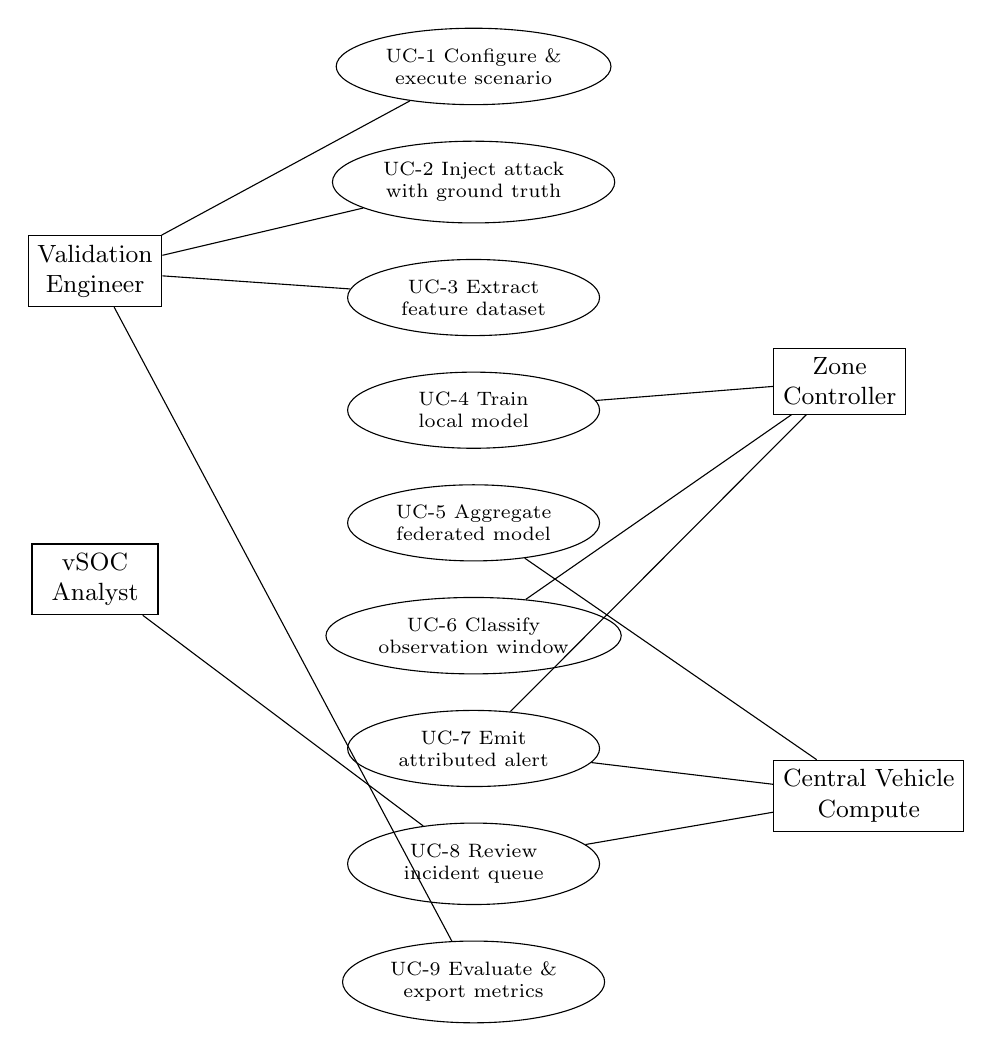
\begin{tikzpicture}[
  actor/.style={draw, minimum width=1.6cm, minimum height=0.6cm, align=center, font=\small},
  uc/.style={draw, ellipse, minimum width=3.2cm, minimum height=0.85cm, align=center, font=\scriptsize},
  node distance=0.45cm and 2.0cm
]
\node[actor] (ve) {Validation\\Engineer};
\node[uc, right=2.2cm of ve, yshift=2.6cm] (uc1) {UC-1 Configure \&\\execute scenario};
\node[uc, below=of uc1] (uc2) {UC-2 Inject attack\\with ground truth};
\node[uc, below=of uc2] (uc3) {UC-3 Extract\\feature dataset};
\node[uc, below=of uc3] (uc4) {UC-4 Train\\local model};
\node[uc, below=of uc4] (uc5) {UC-5 Aggregate\\federated model};
\node[uc, below=of uc5] (uc6) {UC-6 Classify\\observation window};
\node[uc, below=of uc6] (uc7) {UC-7 Emit\\attributed alert};
\node[uc, below=of uc7] (uc8) {UC-8 Review\\incident queue};
\node[uc, below=of uc8] (uc9) {UC-9 Evaluate \&\\export metrics};

\node[actor, right=2.2cm of uc5, yshift=1.8cm] (zc) {Zone\\Controller};
\node[actor, right=2.2cm of uc7, yshift=-0.6cm] (cvc) {Central Vehicle\\Compute};
\node[actor, below=3.0cm of ve] (an) {vSOC\\Analyst};

\draw (ve) -- (uc1); \draw (ve) -- (uc2); \draw (ve) -- (uc3); \draw (ve) -- (uc9);
\draw (an) -- (uc8);
\draw (zc) -- (uc4); \draw (zc) -- (uc6); \draw (zc) -- (uc7);
\draw (cvc) -- (uc5); \draw (cvc) -- (uc7); \draw (cvc) -- (uc8);
\end{tikzpicture}
\caption{Use case diagram. Human actors are shown left, system actors right.}
\label{fig:usecase}
\end{figure}

\section{Detailed Use Cases}

\begin{longtable}{p{0.2\textwidth} p{0.74\textwidth}}
\toprule
\multicolumn{2}{l}{\textbf{UC-2: Inject attack with ground truth}} \\
\midrule
\endfirsthead
Actor & Validation Engineer \\
Precondition & A valid topology and benign baseline configuration exist \\
Trigger & Engineer selects an attack configuration and seed \\
Main flow &
(1) Engineer selects attack class, target zone, start time, intensity and seed.
(2) Simulation executes with injection active over the specified interval.
(3) Harness records, for every observation window, the attack class and the set of
affected zones.
(4) Raw per-node vectors and the ground-truth record are written to the results
directory. \\
Postcondition & A seeded, reproducible run with labels attributable to class, window
and zone \\
Exception & If the attack produces no measurable deviation from baseline, the run is
flagged for parameter review rather than silently retained \\
\bottomrule
\end{longtable}

\begin{longtable}{p{0.2\textwidth} p{0.74\textwidth}}
\toprule
\multicolumn{2}{l}{\textbf{UC-6: Classify observation window}} \\
\midrule
\endfirsthead
Actor & Zone Controller \\
Precondition & A trained global model is deployed locally \\
Trigger & A complete observation window of local TSN signals is available \\
Main flow &
(1) Controller computes the feature vector for the window.
(2) Vector is passed to the local copy of the global model.
(3) Model returns a class and a confidence value.
(4) If the class is not benign for $k$ consecutive windows, an alert is raised. \\
Postcondition & Either no action, or an attributed alert \\
Exception & If no valid model is available, the rule-based fallback detector operates
and the degraded state is made visible \\
\bottomrule
\end{longtable}

\section{Functional Requirements}

\subsection{Module 1: Simulation and Attack Injection}
\begin{itemize}
\item \textbf{FR-01.} The system shall instantiate a configurable multi-zone TSN
topology comprising a grandmaster, a backbone switch, $N$ zone controllers, endpoint
ECUs and a central vehicle compute node.
\item \textbf{FR-02.} The system shall synchronise all time-aware nodes using gPTP.
\item \textbf{FR-03.} The system shall execute reproducibly: a given configuration and
seed shall regenerate the same scenario structure and ground-truth labels.
\item \textbf{FR-04.} The system shall generate benign traffic and at least two
attack classes against TSN synchronisation.
\item \textbf{FR-05.} The system shall record, for every injected attack, the attack
class, the affected zone(s), and the start and end time of the attack interval.
\end{itemize}

\subsection{Module 2: Feature Extraction}
\begin{itemize}
\item \textbf{FR-06.} The system shall convert raw per-node simulation output into
fixed-size observation windows.
\item \textbf{FR-07.} The system shall compute, per window per zone, protocol-native
timing features including clock offset statistics, sibling offset residual, and
synchronisation interval residual.
\item \textbf{FR-08.} The system shall label each window with its attack class and
shall attribute the label to the affected zone(s) only.
\item \textbf{FR-09.} The system shall export the labelled dataset in a documented
schema with a stable column contract.
\item \textbf{FR-10.} Feature extraction shall be passive and shall not alter
forwarding behaviour in the simulated network.
\end{itemize}

\subsection{Module 3: Detection and Federation}
\begin{itemize}
\item \textbf{FR-11.} The system shall train a multiclass detection model on the
labelled feature dataset.
\item \textbf{FR-12.} The system shall support training in three configurations,
namely local-only per zone, centralized pooled, and federated (FedAvg), using an identical
model architecture and identical scenario splits.
\item \textbf{FR-13.} The federated coordinator shall receive model parameters only;
raw feature records shall not leave the client.
\item \textbf{FR-14.} The system shall classify an observation window into benign or a
specific attack class and shall return a confidence value.
\item \textbf{FR-15.} The system shall provide a rule-based fallback detector that
operates when no valid model or coordinator is available, and shall make the degraded
state visible.
\end{itemize}

\subsection{Module 4: Alerting and Evaluation}
\begin{itemize}
\item \textbf{FR-16.} The system shall emit alerts containing attack class, affected
zone, time window, confidence and supporting feature values.
\item \textbf{FR-17.} The system shall present alerts through an operator-facing
incident queue supporting filtering by attack class, severity and status.
\item \textbf{FR-18.} The system shall export machine-readable evaluation metrics
linked to the configuration, seed and model version that produced them.
\end{itemize}

\section{Non-Functional Requirements}

\subsection{Reliability}
\begin{itemize}
\item \textbf{NFR-01.} A documented configuration and seed shall regenerate the same
scenario structure and ground-truth labels on a clean environment.
\item \textbf{NFR-02.} Loss of the coordinator or of a valid model shall produce a
visible fallback state rather than silent cessation of monitoring.
\end{itemize}

\subsection{Usability}
\begin{itemize}
\item \textbf{NFR-03.} An operator shall be able to execute a scenario, extract
features and inspect results from documented commands without modifying source code.
\item \textbf{NFR-04.} Each alert shall carry sufficient attribution for an analyst to
identify the affected zone and time window without consulting raw simulation output.
\end{itemize}

\subsection{Performance}
\begin{itemize}
\item \textbf{NFR-05.} Local classification of one observation window shall complete
within one observation interval on the target workstation.
\item \textbf{NFR-06.} Detection shall occur within a bounded number of
synchronisation intervals from attack onset, and this latency shall be reported in
sync intervals rather than wall-clock seconds.
\end{itemize}

\subsection{Security}
\begin{itemize}
\item \textbf{NFR-07.} Raw feature records shall not be transmitted to the
coordinator; only model parameters and training metadata shall be exchanged.
\item \textbf{NFR-08.} Passive monitoring shall not increase protected-stream
99th-percentile latency by more than 5\% in matched enabled/disabled simulation runs.
\end{itemize}

% [[VERIFY]] NFR-08 is carried over from the approved proposal and is NOT yet
% measured. It is reported as planned in Section 9.5. Do not claim it as met.

\section{Acceptance Criteria}

\begin{longtable}{p{0.1\textwidth} p{0.84\textwidth}}
\toprule
\textbf{Req.} & \textbf{Objective acceptance check} \\
\midrule
\endhead
FR-03 & Two executions with identical configuration and seed produce byte-identical
ground-truth label files. \\
FR-05 & For each attack run, the recorded attack interval matches the interval over
which the timing deviation is observable in the raw trace. \\
FR-07 & For a benign run, the sibling offset residual remains within the documented
benign envelope for all zones across all seeds. \\
FR-08 & For an attack run targeting zone $z$, windows in zone $z$ carry the attack
label and windows in all other zones carry the benign label. \\
FR-10 & Protected-stream latency distributions from matched monitoring-enabled and
monitoring-disabled runs are statistically indistinguishable within the NFR-08 bound. \\
FR-12 & All three training configurations run to completion on identical splits and
produce comparable metric files. \\
FR-13 & Inspection of coordinator-bound messages confirms that no feature record
fields are present. \\
NFR-06 & Measured detection latency is lower than the latency at which accumulated
offset exceeds the configured schedule margin, across all seeds. \\
\bottomrule
\end{longtable}

\section{Requirements Traceability}

\begin{longtable}{p{0.08\textwidth} p{0.14\textwidth} p{0.2\textwidth} p{0.22\textwidth} p{0.22\textwidth}}
\caption{Requirements traceability matrix}\label{tab:traceability}\\
\toprule
\textbf{Req.} & \textbf{Module} & \textbf{Design element} & \textbf{Implementation} & \textbf{Test} \\
\midrule
\endfirsthead
\toprule
\textbf{Req.} & \textbf{Module} & \textbf{Design element} & \textbf{Implementation} & \textbf{Test} \\
\midrule
\endhead
FR-01 & M1 & Sec.~5.1, Fig.~\ref{fig:topology} & \texttt{CarazoneZonalNetwork.ned} & TC-01 \\
FR-02 & M1 & Sec.~5.2 & gPTP configuration in \texttt{omnetpp.ini} & TC-02 \\
FR-03 & M1 & Sec.~5.4 & Seeded run configurations & TC-03 \\
FR-04 & M2 & Sec.~5.8 & \texttt{DelayAttack}, \texttt{DriftAttack}, \texttt{SyncStarvation} & TC-04 \\
FR-05 & M2 & Sec.~5.7 & Ground-truth record & TC-05 \\
FR-06 & M3 & Sec.~5.8, Fig.~\ref{fig:activity} & \texttt{extract\_features.py} & TC-06 \\
FR-07 & M3 & Sec.~5.6 & \texttt{extract\_features.py} & TC-07 \\
FR-08 & M3 & Sec.~5.7 & \texttt{extract\_features.py} & TC-08 (DEF-01) \\
FR-09 & M3 & Table~\ref{tab:schema} & \texttt{features.csv} & TC-09 \\
FR-11--FR-15 & M4, M5 & Sec.~5.1--5.3 & Planned, Iteration 03 & Planned \\
FR-16--FR-18 & M6 & Sec.~5.1 & Planned, Iteration 04 & Planned \\
\bottomrule
\end{longtable}

% ============================================================

\chapter{System Design}
\label{ch:design}
% ============================================================

\section{System Architecture}
\label{sec:architecture}

The system is organised into five layers with explicit interface contracts between
them. Layer separation is deliberate: the simulation layer is replaceable by captured
traces from a hardware testbed, and the detection layer is replaceable by a different
model, without either change propagating beyond its own interface.

\begin{figure}[htbp]
\centering
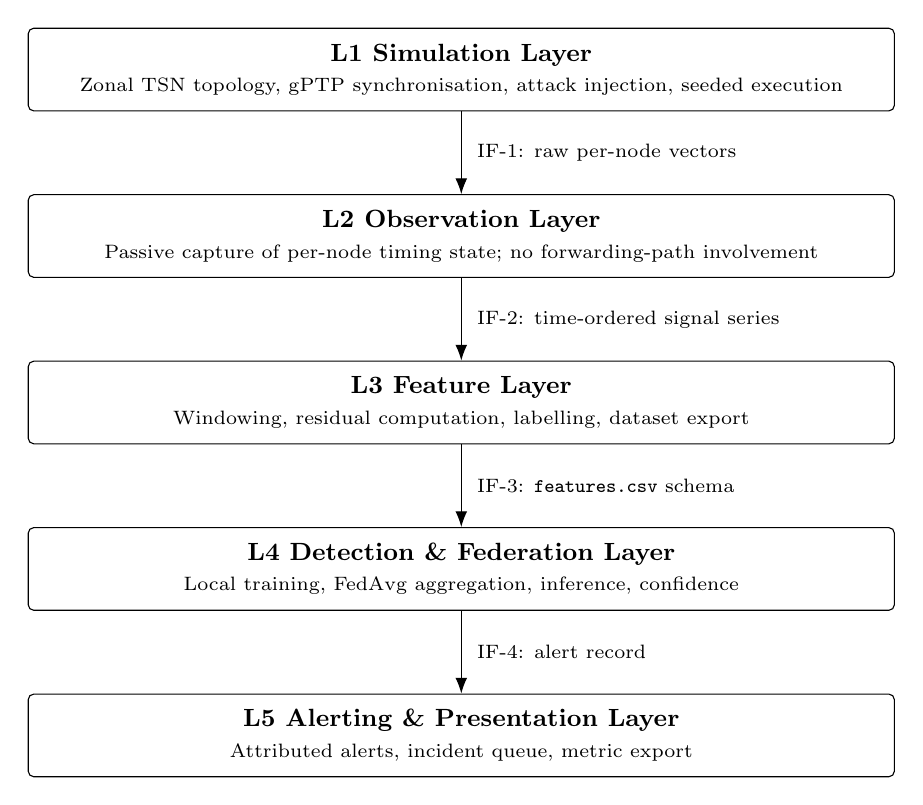
\begin{tikzpicture}[
  layer/.style={draw, rounded corners=2pt, minimum width=11cm, minimum height=1.05cm,
                align=center, font=\small},
  iface/.style={font=\scriptsize, align=center},
  node distance=1.05cm
]
\node[layer] (l1) {\textbf{L1 Simulation Layer} \\
  \scriptsize Zonal TSN topology, gPTP synchronisation, attack injection, seeded execution};
\node[layer, below=of l1] (l2) {\textbf{L2 Observation Layer} \\
  \scriptsize Passive capture of per-node timing state; no forwarding-path involvement};
\node[layer, below=of l2] (l3) {\textbf{L3 Feature Layer} \\
  \scriptsize Windowing, residual computation, labelling, dataset export};
\node[layer, below=of l3] (l4) {\textbf{L4 Detection \& Federation Layer} \\
  \scriptsize Local training, FedAvg aggregation, inference, confidence};
\node[layer, below=of l4] (l5) {\textbf{L5 Alerting \& Presentation Layer} \\
  \scriptsize Attributed alerts, incident queue, metric export};

\draw[-{Latex[length=2mm]}] (l1) -- node[right, iface] {\;IF-1: raw per-node vectors} (l2);
\draw[-{Latex[length=2mm]}] (l2) -- node[right, iface] {\;IF-2: time-ordered signal series} (l3);
\draw[-{Latex[length=2mm]}] (l3) -- node[right, iface] {\;IF-3: \texttt{features.csv} schema} (l4);
\draw[-{Latex[length=2mm]}] (l4) -- node[right, iface] {\;IF-4: alert record} (l5);
\end{tikzpicture}
\caption{Layered system architecture with interface contracts.}
\label{fig:arch}
\end{figure}

\section{Architectural Components}
\label{sec:components}

\begin{longtable}{p{0.18\textwidth} p{0.24\textwidth} p{0.5\textwidth}}
\toprule
\textbf{Component} & \textbf{Layer} & \textbf{Responsibility} \\
\midrule
\endhead
Topology model & L1 & Declares nodes, links and per-node clock configuration \\
Scenario manager & L1 & Schedules attack events at configured times and targets \\
gPTP instances & L1 & Distribute time from the grandmaster through the relay tree \\
Signal recorder & L2 & Records per-node clock state at sample points \\
Window builder & L3 & Segments series into fixed-size observation windows \\
Feature computer & L3 & Computes per-window statistics and residuals \\
Labeller & L3 & Assigns class and zone attribution from the ground-truth record \\
Local trainer & L4 & Trains the shared model architecture on a client's local dataset \\
Aggregator & L4 & Performs FedAvg over received parameters \\
Inference engine & L4 & Classifies windows using the deployed global model \\
Fallback detector & L4 & Rule-based detection when no valid model is available \\
Alert builder & L5 & Constructs attributed alert records \\
Incident queue & L5 & Operator-facing triage surface \\
\bottomrule
\end{longtable}

\section{Interfaces and Dependencies}
\label{sec:interfaces}

\begin{longtable}{p{0.08\textwidth} p{0.26\textwidth} p{0.58\textwidth}}
\toprule
\textbf{ID} & \textbf{Interface} & \textbf{Contract} \\
\midrule
\endhead
IF-1 & Simulation $\rightarrow$ Observation &
Per-node recorded vectors in the simulator's result format; one vector per node per
run; node identity encoded in the vector name \\
\addlinespace
IF-2 & Observation $\rightarrow$ Feature &
Time-ordered $(t, \text{value})$ series per node, with run identifier and seed \\
\addlinespace
IF-3 & Feature $\rightarrow$ Detection &
\texttt{features.csv} column contract (Table~\ref{tab:schema}); one row per window per
zone; stable column order; documented units \\
\addlinespace
IF-4 & Detection $\rightarrow$ Alerting &
Alert record: \{class, confidence, zone, window start, window end, run id,
supporting feature values\} \\
\addlinespace
IF-5 & Client $\leftrightarrow$ Coordinator &
Model parameters and training metadata (sample count, round index). Feature records
are explicitly excluded from this interface (NFR-07) \\
\bottomrule
\end{longtable}

\textbf{External dependencies.} OMNeT++ 6.4.0 (simulation kernel, Qtenv/Cmdenv),
INET 4.7.0~\cite{inettsn} (TSN and gPTP modules), Python 3 with scientific stack for extraction and
training, and a federated learning framework for the aggregation layer. Versions are
pinned in Section~\ref{sec:dependencies}.

\section{Architecture Decisions and Rationale}
\label{sec:arch-decisions}

\begin{longtable}{p{0.06\textwidth} p{0.26\textwidth} p{0.26\textwidth} p{0.34\textwidth}}
\caption{Architecture decision record}\\
\toprule
\textbf{ID} & \textbf{Decision} & \textbf{Alternatives considered} & \textbf{Rationale} \\
\midrule
\endfirsthead
\toprule
\textbf{ID} & \textbf{Decision} & \textbf{Alternatives considered} & \textbf{Rationale} \\
\midrule
\endhead
AD-1 & Use OMNeT++/INET as the simulation framework &
Build a custom simulator; use a hardware TSN testbed; use a generic network simulator
without TSN modules &
INET provides gPTP, time-aware shaping and clock-drift modelling as maintained
components, and its TSN capabilities have been verified against TSN hardware
measurements in published work. Building a simulator would consume the project budget
without advancing the research question. A hardware testbed is unavailable and its
procurement risk is unacceptable within the timeline. \\
\addlinespace
AD-2 & Supervised multiclass classification &
Unsupervised (LOF, autoencoder, Deep SVDD); two-stage hybrid &
Simulation supplies ground-truth labels, removing the label-scarcity constraint that
motivates unsupervised framing in the comparable literature. A parametric model has
trainable weights and is therefore FedAvg-compatible without a non-standard
aggregation scheme; LOF is not. LOF is retained as a comparison baseline for
comparability with published results. \\
\addlinespace
AD-3 & Federate across zones within one vehicle &
Federate across vehicles/fleet &
The aggregation server is the vehicle's own central compute unit. Within-vehicle
federation is motivated by backbone bandwidth, not inter-organisational privacy:
periodic fixed-size parameter exchange is a bounded, schedulable traffic pattern,
whereas continuous trace upload is unbounded best-effort traffic competing with
protected streams. \\
\addlinespace
AD-4 & Static, one-shot training &
Continuous/online federated learning &
Online retraining in deployment requires live ground-truth labelling, which has no
solution within scope. Assumption A2. \\
\addlinespace
AD-5 & Static network environment assumption &
Support runtime reconfiguration &
The detection approach computes residuals against an expected value known from
configuration. This is available \emph{a priori} only when the configuration is
static. Supporting dynamic reconfiguration requires distinguishing legitimate
reconfiguration from attack, which is a separate research problem. Assumption A1. \\
\addlinespace
AD-6 & Detector positioned at the zone controller &
Position at endpoint ECU; position centrally &
The primary features require simultaneous visibility of multiple ports: the sibling
offset residual cannot be computed by a node that observes only its own clock. The
zone controller is the lowest point in the hierarchy with the required visibility. \\
\addlinespace
AD-7 & Flat CSV dataset with a documented column contract rather than a relational
schema &
Relational database with entity-relationship model &
The data is a single homogeneous observation table with no multi-entity relational
structure. A relational model would add no referential integrity benefit and would
not reflect the domain. Section~\ref{sec:data-design} therefore specifies a column contract rather than
an ERD. \\
\bottomrule
\end{longtable}

\section{Reference Topology Design}
\label{sec:ref-topology}

The Iteration~1 results reported in Chapter~\ref{ch:testing} were produced on a four-zone tree
topology, described in Section~\ref{sec:technical-details} and retained as \texttt{topology\_basic}. That
topology was built to be minimal: it was enough to instrument gPTP, inject delay
attacks and test the cross-zone residual claim, and deliberately no more. It has two
properties that bound what can be asked of it. Each zone reaches the backbone over a
single path, so FRER cannot be configured, and all four zones carry identical traffic,
which is recorded as defect DEF-02.

A second topology, \texttt{topology5}, has since been designed and generated to remove
both limits. It is the reference topology for the remainder of the project. It has
been validated structurally but has not yet produced a dataset, so no result in this
report is derived from it.

\subsection{Basis of the design}
No vehicle manufacturer publishes harness or ECU-placement data, so the topology is
built as a representative reference rather than a copy of a production vehicle. Three
published sources inform it. The zone-based in-vehicle architecture evaluated in
\emph{Sensors}~\cite{park2023zonal} supplies the organising principle: ECUs are grouped into zones
by physical location, attached to the nearest zone controller, with a central compute
unit as the inter-zone hub. The TSN anomaly-detection assessment framework of
Meyer, H\"ackel, L\"ubeck, Korf and Schmidt~\cite{meyer2024framework} supplies a precedent for a
ring-based zonal topology carrying
corner lidar, front and rear cameras, infotainment, a connectivity gateway, a gPTP
master and an ADAS unit, modelled in OMNeT++/INET. Industry material on zonal E/E
architecture, including the IEEE~802 zonal presentation and Excelfore's TSN wheel-sensor
work, supplies the four-corner-plus-cabin arrangement and the use of TSN for
time-critical traffic with network redundancy. The device list is the project's own
representative model and is not claimed to match any production vehicle.

\subsection{Zone partitioning}
The vehicle is divided into five zones: front-left (FL), front-right (FR), rear-left
(RL), rear-right (RR) and a centre/cabin zone (C). Each zone has one TSN switch and
one zonal controller host, and the controller is the node that runs the local detector
and acts as the federated client. Devices are assigned to zones by three rules applied
in order: physical proximity, so a device connects to the switch of the zone in which
it is mounted; safety separation, so safety-critical actuators such as steering and
brake are kept apart from infotainment and external-facing nodes; and a load limit, so
a zone's uplink load stays within the capacity of its links, with devices moved or link
speed revisited if it does not.

The model contains 25 endpoint ECUs, five zonal controllers, a central compute unit, a
connectivity gateway and a gPTP master clock.

\begin{longtable}{p{0.16\textwidth} r p{0.56\textwidth}}
\caption{Zone composition of the reference topology}\label{tab:topology5}\\
\toprule
\textbf{Zone} & \textbf{ECUs} & \textbf{Examples} \\
\midrule
\endfirsthead
\toprule
\textbf{Zone} & \textbf{ECUs} & \textbf{Examples} \\
\midrule
\endhead
Front-left & 7 & lidar, radar, front camera, left mirror camera, steering, brake,
front ultrasonic \\
Front-right & 6 & lidar, radar, right mirror camera, powertrain, ultrasonic,
headlamp \\
Rear-left & 3 & lidar, radar, ultrasonic \\
Rear-right & 4 & lidar, radar, rear camera, V2X unit \\
Centre/cabin & 5 & infotainment, instrument cluster, driver-monitoring camera,
audio amplifier, GNSS receiver \\
\bottomrule
\end{longtable}

The distribution is deliberately uneven. The front zones carry dense sensing and
control traffic, the rear zones are lighter, and the cabin zone carries mainly
multimedia and display traffic. The ECU count was chosen for this project rather than
copied from the source architecture: enough devices per zone to give each federated
client a meaningful local dataset, while keeping the simulation maintainable.

\subsection{Interconnect}
Within a zone, devices connect to the zone switch in a star. Between zones, the four
corner switches form a ring (FL, FR, RR, RL) and the centre switch is dual-homed to
both front switches. Every zone therefore has two link-disjoint routes to the centre,
which is precisely the property that Frame Replication and Elimination for Reliability
requires and which the earlier tree topology could not provide. Ring links and ADAS
sensors run at 1~Gbps; lower-rate ECUs run at 100~Mbps. Link lengths of 0.5 to 3.5~m
are assumed values chosen to be plausible for a passenger vehicle and are kept below
the 15~m reach of automotive Ethernet over unshielded twisted pair.

The ring is the primary topology because it enables FRER-based detection features and
path-change behaviour in gPTP. A star topology over the same device inventory is
retained as a baseline for comparison, since a star offers only one path per zone and
therefore isolates what the redundancy actually contributes.

\subsection{Time synchronisation}
A gPTP grandmaster is attached to the centre switch. Synchronisation follows a static
tree: grandmaster, centre switch, front switches, rear switches, then end devices. The
two ring links not on this tree (FL to FR, and RL to RR) carry no synchronisation
messages. The simulator's gPTP implementation assigns master and slave ports statically
and has no best-master-clock algorithm, so a backup grandmaster is not modelled within
the current scope. gPTP and FRER are the two TSN signals used for detection.

\subsection{Generation and reproducibility}
The network description (\texttt{.ned}), the simulation configuration
(\texttt{omnetpp.ini}) and the validation checks are all generated from a single Python
table of devices, link speeds and link lengths (\texttt{gen\_topology.py}). Editing the
table and re-running the generator regenerates both simulator files, so the model
cannot drift out of step with its own specification, and the generation step runs in
the project's continuous integration pipeline (Section~\ref{sec:repository}).

\begin{figure}[htbp]
\centering
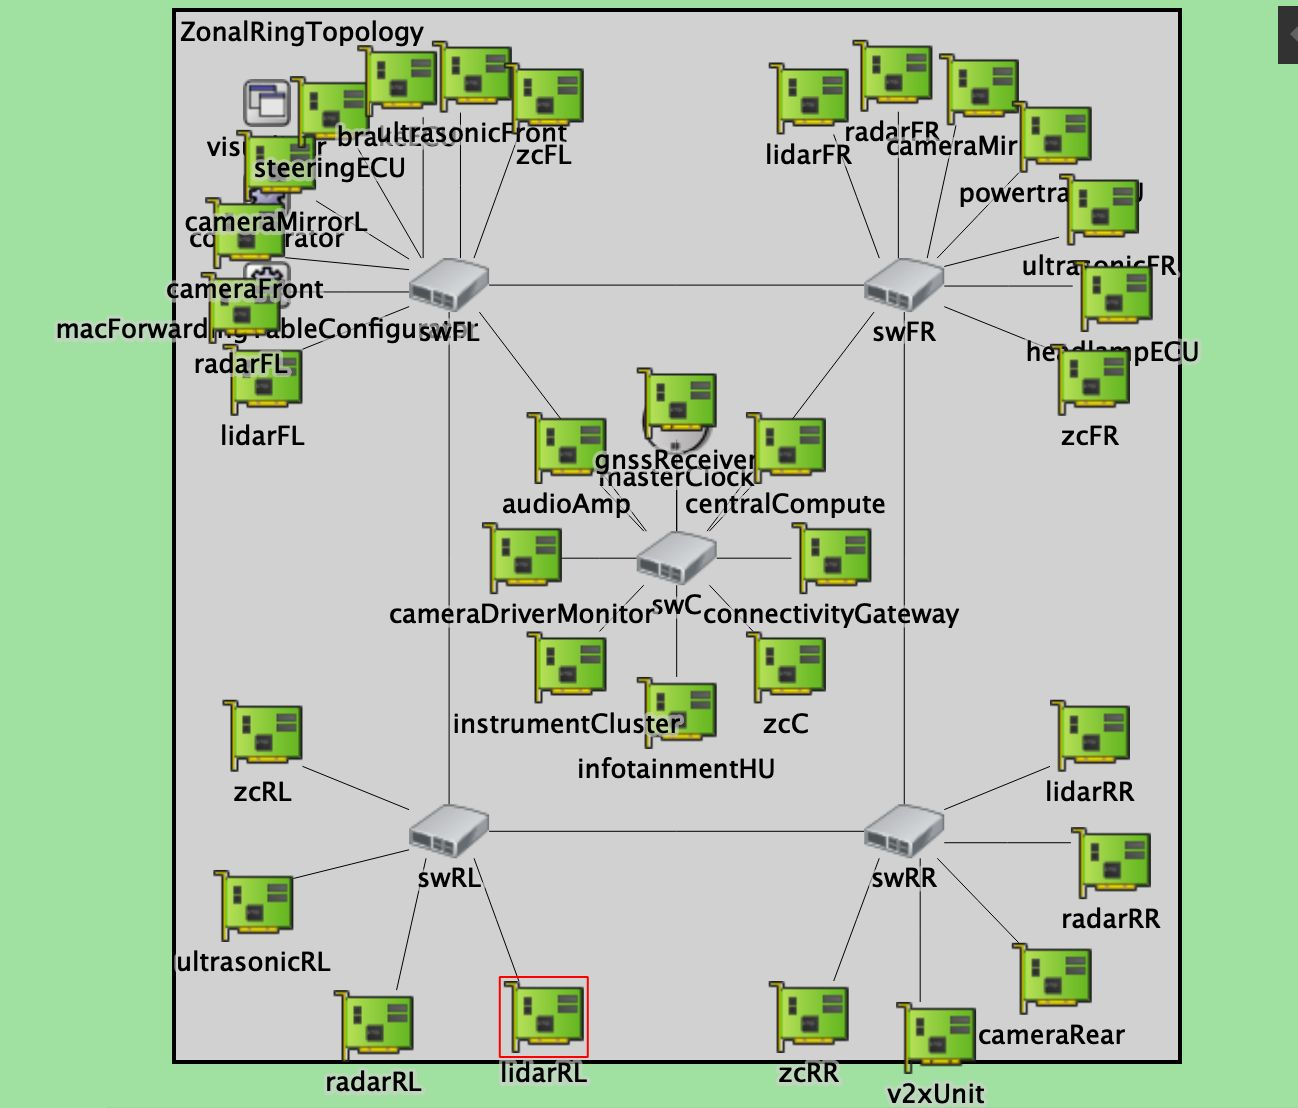
\includegraphics[width=0.95\textwidth]{figures/network_topology.jpeg}
\caption[Five-zone ring reference topology]{The five-zone ring reference topology (\texttt{ZonalRingTopology}) as
rendered in the simulator. The four corner switches \texttt{swFL}, \texttt{swFR},
\texttt{swRR} and \texttt{swRL} form the ring; the centre switch \texttt{swC} is
dual-homed to both front switches. Every zone therefore has two link-disjoint routes
to the centre, which is the property FRER requires. Each zone switch carries its own
zonal controller (\texttt{zcFL}, \texttt{zcFR}, \texttt{zcRL}, \texttt{zcRR},
\texttt{zcC}), which is the node that acts as a federated client, together with the
endpoint ECUs of that zone. The grandmaster (\texttt{masterClock}) and the central
compute unit are attached to \texttt{swC}.}\label{fig:topology5}
\end{figure}

\subsection{Validation}
\label{sec:topology-validation}
The topology is checked at three levels.

\textbf{Structural, automated.} The generator verifies that the graph is connected,
that each endpoint has exactly one switch port, that cutting any single ring or uplink
link partitions nothing, and that every link is shorter than 15~m. The current model
passes all of these checks. The partition check is the one that matters for FRER: it is
the machine-checkable form of the disjoint-path requirement.

\textbf{Physical plausibility, manual.} Each device is checked against the placement
rules: sensors connect to the switch of the zone in which they are mounted, cabin
devices connect to the front or centre zone, and safety-critical ECUs are kept separate
from infotainment. Each placement is justified by a source or a stated reason.

\textbf{Network behaviour, simulation.} The third level is specified here as the
acceptance criteria for the benign baseline run, which is the first task of
Iteration~03c (Section~\ref{sec:remaining-iterations}). The topology is accepted as behaviourally sound when all
time-triggered flows meet their deadlines, link utilisation stays below approximately
70\%, gPTP converges within the target bound, and FRER flows survive a cut ring link.
Stating these criteria before the run is deliberate: it fixes what counts as a
successful topology in advance, so that the baseline run tests the design rather than
being read as a description of whatever it happens to produce.

\subsection{Expected heterogeneity}
Each zonal controller acts as a federated client whose data is the traffic passing
through its zone switch. The topology is designed so that three kinds of non-IID
behaviour can arise across those clients: quantity skew, since zones differ in the
number of flows and therefore in the number of samples; feature skew, since traffic
classes, packet sizes and rates differ by zone and gPTP delay grows with hop distance
from the grandmaster; and label skew, since attack exposure differs by zone, with
V2X-related attacks reaching the rear-right zone and gPTP attacks affecting deeper
zones more strongly.

This is the designed remedy for defect DEF-02, which records that the four zones of the
earlier topology carry identical traffic and would make the federated comparison null
by construction. The remedy is a design property until it is measured. It will be
quantified by comparing per-zone feature distributions, using the
Kolmogorov--Smirnov statistic or the Wasserstein distance, and per-zone label
distributions, using the Jensen--Shannon divergence. Until those numbers exist, DEF-02
is reduced from open to partially addressed rather than closed.

\subsection{Limitations}
Four limitations are recorded against this topology. The device list and link lengths
are representative rather than taken from a manufacturer's vehicle. The model carries no
application traffic yet, so the heterogeneity described above is a design property and
not a measured one. gPTP is statically configured with no backup grandmaster, so
grandmaster-failover behaviour cannot be exercised. Some zone switches have ten or
eleven ports, which is higher than a typical automotive TSN switch; they are best read
as zonal controllers with integrated switching rather than as discrete switches.

\section{Design Evolution}

Six design changes have occurred since the approved proposal, each with its
justification:

\begin{longtable}{p{0.22\textwidth} p{0.24\textwidth} p{0.46\textwidth}}
\toprule
\textbf{Element} & \textbf{Proposal $\rightarrow$ Current} & \textbf{Justification} \\
\midrule
\endhead
Number of federated clients & Three $\rightarrow$ Four &
Followed from the zonal topology design, which maps a client to a physical zone
rather than to an arbitrary partition. Client count remains a configuration parameter. \\
\addlinespace
Attack classes & Sync manipulation and delay injection $\rightarrow$ delay injection,
sync starvation, drift (evaluated and excluded) &
Sync starvation is a concrete realisation of synchronisation manipulation. Drift
manipulation was implemented and empirically found not to produce a zone-localisable
signature (Section~\ref{sec:edge-cases}); it is retained in the report as a documented negative
result rather than as a detection target. \\
\addlinespace
Reference topology & Four-zone tree $\rightarrow$ five-zone ring with dual-homed
centre &
The tree was minimal by design and sufficient to test the residual claim, but it
offers one path per zone and so cannot carry FRER. The ring gives every zone two
link-disjoint routes to the centre. Specified in Section~\ref{sec:ref-topology}; Iteration~1 results in
Chapter~\ref{ch:testing} remain those of the tree. \\
\addlinespace
Federated client count & Four $\rightarrow$ five &
Follows the reference topology, which has five zones rather than four. The client
count is a property of the topology, not an independent parameter. \\
\addlinespace
FRER-based detection & Not in proposal $\rightarrow$ committed scope, in progress &
Added to the attack surface after the proposal, to test whether the cross-zone
residual principle generalises beyond the synchronisation plane. Blocked on a single
dependency, the absence of disjoint paths in the Iteration~1 tree, which the
five-zone ring topology now resolves. The 802.1CB configuration and feature family
are scheduled in Section~\ref{sec:remaining-iterations}. \\
\addlinespace
Team composition & Three-member ownership model $\rightarrow$ two members &
Responsibilities reallocated across two members (Section~\ref{sec:workbreakdown}); each member retains a
distinct primary implementation area. \\
\bottomrule
\end{longtable}

\section{Domain Model}
\label{sec:domain-model}

The domain is described by seven concepts. The synchronisation tree structure is
central: the sibling relationship between zones at the same depth is what makes the
residual feature computable, and its absence is what makes a grandmaster-level
perturbation undetectable by this approach.

\begin{figure}[htbp]
\centering
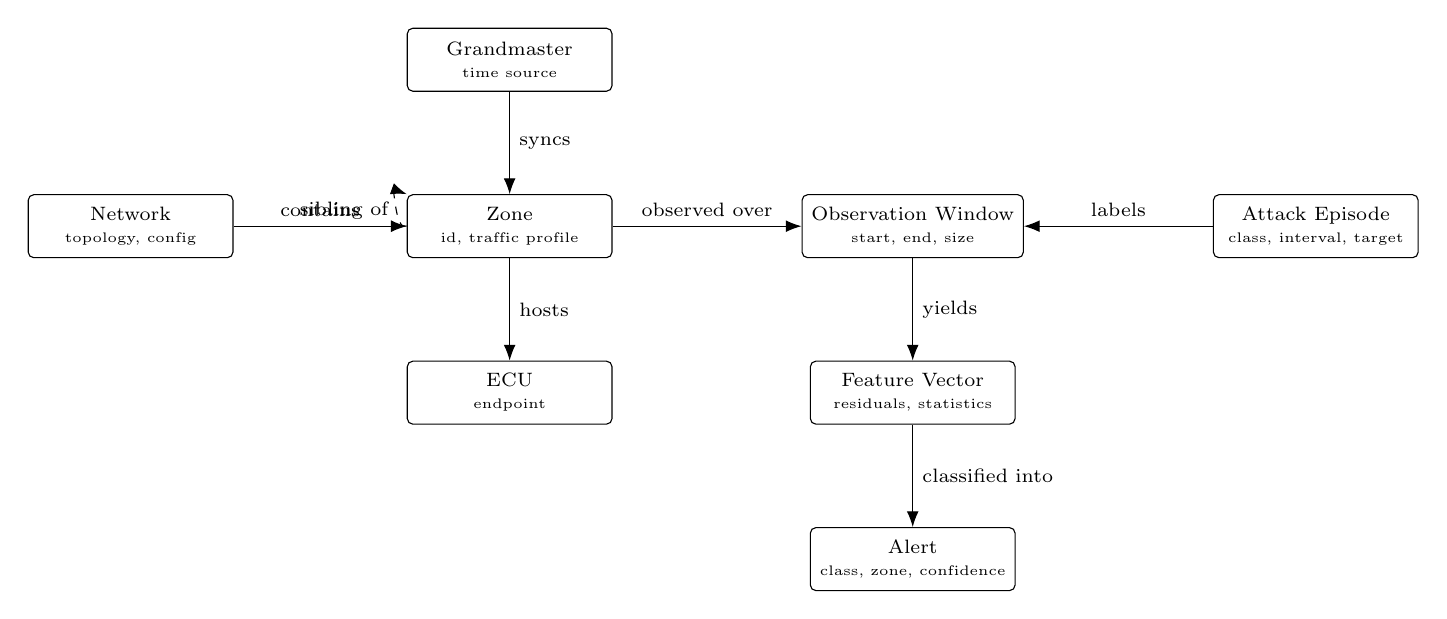
\begin{tikzpicture}[
  ent/.style={draw, rounded corners=2pt, minimum width=2.6cm, minimum height=0.8cm,
              align=center, font=\scriptsize},
  rel/.style={font=\scriptsize, midway}
]
\node[ent] (gm) {Grandmaster\\\tiny time source};
\node[ent, below=1.3cm of gm] (zone) {Zone\\\tiny id, traffic profile};
\node[ent, left=2.2cm of zone] (net) {Network\\\tiny topology, config};
\node[ent, below=1.3cm of zone] (ecu) {ECU\\\tiny endpoint};
\node[ent, right=2.4cm of zone] (obs) {Observation Window\\\tiny start, end, size};
\node[ent, below=1.3cm of obs] (fv) {Feature Vector\\\tiny residuals, statistics};
\node[ent, right=2.4cm of obs] (att) {Attack Episode\\\tiny class, interval, target};
\node[ent, below=1.3cm of fv] (al) {Alert\\\tiny class, zone, confidence};

\draw[-{Latex[length=2mm]}] (gm) -- node[rel, right] {syncs} (zone);
\draw[-{Latex[length=2mm]}] (net) -- node[rel, above] {contains} (zone);
\draw[-{Latex[length=2mm]}] (zone) -- node[rel, right] {hosts} (ecu);
\draw[-{Latex[length=2mm]}] (zone) -- node[rel, above] {observed over} (obs);
\draw[-{Latex[length=2mm]}] (obs) -- node[rel, right] {yields} (fv);
\draw[-{Latex[length=2mm]}] (att) -- node[rel, above] {labels} (obs);
\draw[-{Latex[length=2mm]}] (fv) -- node[rel, right] {classified into} (al);
\draw[-{Latex[length=2mm]}, dashed] (zone.west) to[out=200,in=160]
      node[rel, left] {sibling of} (zone.north west);
\end{tikzpicture}
\caption[Domain model]{Domain model. The dashed self-relation on Zone is the sibling relationship
within the synchronisation tree, on which the residual feature depends.}
\label{fig:domain}
\end{figure}

\section{Data Design}
\label{sec:data-design}

The system does not use a relational database. Its persistent data is a single
homogeneous observation table together with run metadata, so the data design is
specified as a column contract rather than an entity-relationship model (decision
AD-7).

\begin{longtable}{p{0.26\textwidth} p{0.12\textwidth} p{0.1\textwidth} p{0.42\textwidth}}
\caption{\texttt{features.csv} column contract}\label{tab:schema}\\
\toprule
\textbf{Column} & \textbf{Type} & \textbf{Unit} & \textbf{Description} \\
\midrule
\endfirsthead
\multicolumn{4}{l}{\textit{Table \thetable{} continued from previous page}}\\
\toprule
\textbf{Column} & \textbf{Type} & \textbf{Unit} & \textbf{Description} \\
\midrule
\endhead
\multicolumn{4}{l}{\textit{Identity and labelling}}\\
\texttt{run} & string & n/a & Run identifier assigned by the simulator, unique per
configuration and seed \\
\texttt{config} & string & n/a & Configuration name: \texttt{Benign},
\texttt{DelayAttack}, \texttt{DriftAttack} or \texttt{SyncStarvation} \\
\texttt{zone} & int & n/a & Zone index, $0 \ldots N-1$ \\
\texttt{target\_zone} & int & n/a & Zone targeted by the attack in this run; empty for
benign runs. Ground truth for attribution, and excluded from every feature set because
it is equivalent to the label \\
\texttt{window\_start} & float & s & Simulation time at window start; window length and
stride are extraction parameters \\
\texttt{label} & int & n/a & Class id: 0 benign, 1 delay, 2 drift, 3 starvation \\
\addlinespace
\multicolumn{4}{l}{\textit{Zone-controller features, prefix} \texttt{ctrl\_}}\\
\texttt{n\_events} & float & count & Number of clock-change events in the window; zero
is retained rather than dropped, as absence of events is itself the signature of sync
starvation \\
\texttt{mean\_offset} & float & s & Mean clock offset against ideal time \\
\texttt{std\_offset} & float & s & Standard deviation of offset \\
\texttt{max\_abs\_offset} & float & s & Maximum absolute offset \\
\texttt{offset\_range} & float & s & Peak-to-peak offset \\
\texttt{mean\_abs\_step} & float & s & Mean absolute correction step between
consecutive events \\
\texttt{max\_abs\_step} & float & s & Largest single correction step \\
\texttt{drift\_slope} & float & s/s & Linear slope of offset over the window \\
\addlinespace
\multicolumn{4}{l}{\textit{Zone aggregates over controller and member ECUs, prefixes}
\texttt{zone\_mean\_} \textit{and} \texttt{zone\_std\_}}\\
\texttt{zone\_mean\_\{f\}} & float & n/a & Mean of feature $f$ across all nodes in the
zone, for each of the eight features above \\
\texttt{zone\_std\_\{f\}} & float & n/a & Standard deviation of feature $f$ across all
nodes in the zone \\
\addlinespace
\multicolumn{4}{l}{\textit{Planned, Iteration 03}}\\
\texttt{sibling\_residual} & float & s & Controller mean offset minus the median
controller mean offset of all other zones in the same window. \textbf{Not yet
implemented} \\
\bottomrule
\texttt{sibling\_n\_\{f\}} & float & count & Number of sibling zones that
contributed to the residual for feature $f$ in this window. Recorded so that a residual
computed against a reduced set of siblings can be identified rather than silently
trusted \\
\end{longtable}

\textbf{Offset definition.} Node offset is derived from the simulator's recorded clock
trace as $\mathrm{offset}(t) = \mathrm{clock\_time}(t) - \mathrm{simulation\_time}(t)$,
the node's error against the ideal timeline. Under correct gPTP operation this remains
within a narrow band, punctuated by corrections at each synchronisation interval; each
attack class perturbs that pattern differently.

\textbf{Integrity rules.} (R1) Every window belongs to exactly one run and one zone.
(R2) A window carries an attack class label only if its zone is the designated victim
of the run \emph{and} the attack is active over the window. (R3) Train/test splits are
formed at run and seed granularity, never at window granularity, because the extraction
stride is shorter than the window length and adjacent windows therefore overlap.

\section{Process / Behavior Design}
\label{sec:process-design}

\subsection*{Data flow}

\begin{figure}[htbp]
\centering
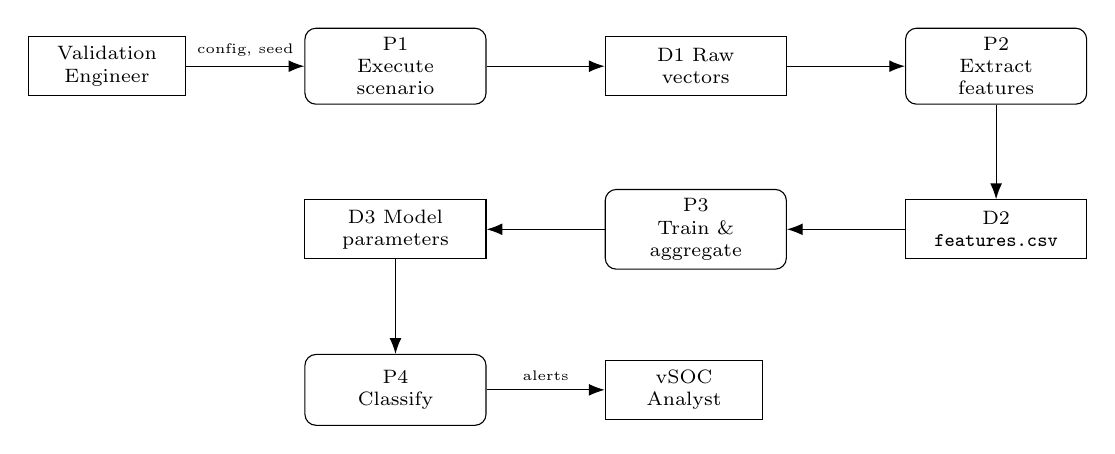
\begin{tikzpicture}[
  proc/.style={draw, rounded corners=4pt, minimum width=2.3cm, minimum height=0.9cm,
               align=center, font=\scriptsize},
  store/.style={draw, minimum width=2.3cm, minimum height=0.75cm, align=center,
                font=\scriptsize},
  ext/.style={draw, minimum width=2.0cm, minimum height=0.75cm, align=center,
              font=\scriptsize},
  node distance=1.4cm
]
\node[ext] (eng) {Validation\\Engineer};
\node[proc, right=1.5cm of eng] (p1) {P1\\Execute\\scenario};
\node[store, right=1.5cm of p1] (d1) {D1 Raw\\vectors};
\node[proc, right=1.5cm of d1] (p2) {P2\\Extract\\features};
\node[store, below=1.2cm of p2] (d2) {D2\\\texttt{features.csv}};
\node[proc, left=1.5cm of d2] (p3) {P3\\Train \&\\aggregate};
\node[store, left=1.5cm of p3] (d3) {D3 Model\\parameters};
\node[proc, below=1.2cm of d3] (p4) {P4\\Classify};
\node[ext, right=1.5cm of p4] (soc) {vSOC\\Analyst};

\draw[-{Latex[length=2mm]}] (eng) -- node[above, font=\tiny] {config, seed} (p1);
\draw[-{Latex[length=2mm]}] (p1) -- (d1);
\draw[-{Latex[length=2mm]}] (d1) -- (p2);
\draw[-{Latex[length=2mm]}] (p2) -- (d2);
\draw[-{Latex[length=2mm]}] (d2) -- (p3);
\draw[-{Latex[length=2mm]}] (p3) -- (d3);
\draw[-{Latex[length=2mm]}] (d3) -- (p4);
\draw[-{Latex[length=2mm]}] (p4) -- node[above, font=\tiny] {alerts} (soc);
\end{tikzpicture}
\caption{Level-1 data flow diagram.}
\label{fig:dfd}
\end{figure}

\subsection*{Feature extraction activity}

\begin{figure}[htbp]
\centering
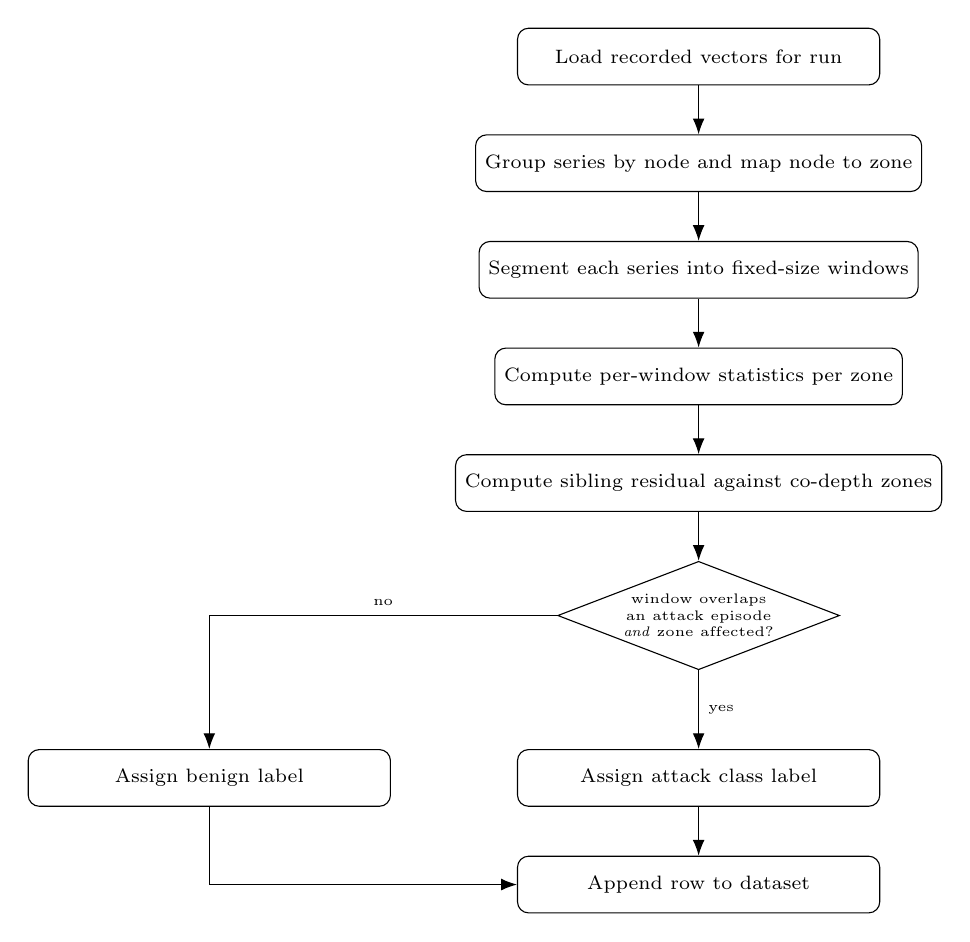
\begin{tikzpicture}[
  act/.style={draw, rounded corners=4pt, minimum width=4.6cm, minimum height=0.72cm,
              align=center, font=\scriptsize},
  dec/.style={draw, diamond, aspect=2.6, inner sep=1pt, align=center, font=\tiny},
  node distance=0.62cm
]
\node[act] (a1) {Load recorded vectors for run};
\node[act, below=of a1] (a2) {Group series by node and map node to zone};
\node[act, below=of a2] (a3) {Segment each series into fixed-size windows};
\node[act, below=of a3] (a4) {Compute per-window statistics per zone};
\node[act, below=of a4] (a5) {Compute sibling residual against co-depth zones};
\node[dec, below=of a5] (d1) {window overlaps\\an attack episode\\\emph{and} zone affected?};
\node[act, below=1.0cm of d1] (a6) {Assign attack class label};
\node[act, left=1.6cm of a6] (a7) {Assign benign label};
\node[act, below=of a6] (a8) {Append row to dataset};

\draw[-{Latex[length=2mm]}] (a1)--(a2); \draw[-{Latex[length=2mm]}] (a2)--(a3);
\draw[-{Latex[length=2mm]}] (a3)--(a4); \draw[-{Latex[length=2mm]}] (a4)--(a5);
\draw[-{Latex[length=2mm]}] (a5)--(d1);
\draw[-{Latex[length=2mm]}] (d1)-- node[right, font=\tiny] {yes} (a6);
\draw[-{Latex[length=2mm]}] (d1.west) -| node[above, font=\tiny, pos=0.25] {no} (a7);
\draw[-{Latex[length=2mm]}] (a6)--(a8);
\draw[-{Latex[length=2mm]}] (a7) |- (a8);
\end{tikzpicture}
\caption[Feature extraction activity]{Feature extraction activity. The decision node implements integrity rule R2:
a window is labelled with the attack class only when its zone is the run's designated
victim and the attack is active. The sibling-residual step is planned for
Iteration~03.}
\label{fig:activity}
\end{figure}

\subsection*{Detector state behaviour}

\begin{figure}[htbp]
\centering
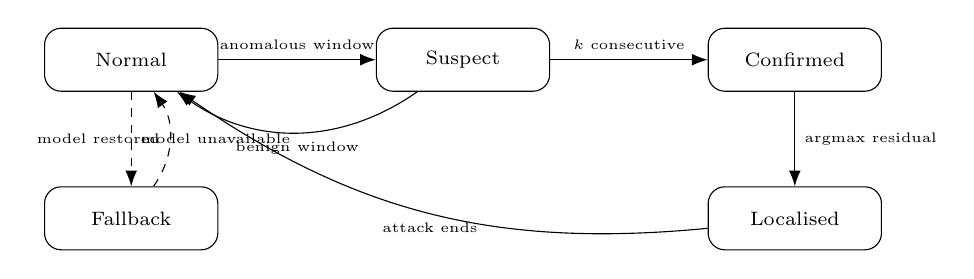
\begin{tikzpicture}[
  st/.style={draw, rounded corners=6pt, minimum width=2.2cm, minimum height=0.8cm,
             align=center, font=\scriptsize},
  node distance=2.0cm
]
\node[st] (n) {Normal};
\node[st, right=of n] (s) {Suspect};
\node[st, right=of s] (c) {Confirmed};
\node[st, below=1.2cm of c] (l) {Localised};
\node[st, below=1.2cm of n] (f) {Fallback};

\draw[-{Latex[length=2mm]}] (n) -- node[above, font=\tiny] {anomalous window} (s);
\draw[-{Latex[length=2mm]}] (s) -- node[above, font=\tiny] {$k$ consecutive} (c);
\draw[-{Latex[length=2mm]}] (s) to[bend left=35] node[below, font=\tiny] {benign window} (n);
\draw[-{Latex[length=2mm]}] (c) -- node[right, font=\tiny] {argmax residual} (l);
\draw[-{Latex[length=2mm]}] (l) to[bend left=20] node[below, font=\tiny] {attack ends} (n);
\draw[-{Latex[length=2mm]}, dashed] (n) -- node[right, font=\tiny] {model unavailable} (f);
\draw[-{Latex[length=2mm]}, dashed] (f) to[bend right=35] node[left, font=\tiny] {model restored} (n);
\end{tikzpicture}
\caption[Detector state machine]{Detector state machine. The $k$-consecutive-window transition implements the
detection-latency requirement NFR-06; the dashed transitions implement FR-15.}
\label{fig:state}
\end{figure}

\subsection*{Attack mechanism}

The asymmetric delay attack exploits the symmetry assumption in the peer-delay
computation. Under normal operation a node computes link delay as
$D = ((t_4 - t_1) - (t_3 - t_2))/2$, which is correct only when the forward and
reverse path delays are equal. An attacker who delays messages in one direction only
introduces an asymmetry $\delta$, producing a link-delay error of $\delta/2$ that
propagates directly into the offset correction. The messages themselves remain
authentic and unmodified, which is why message authentication does not mitigate this
attack class.

% [[FILL]] A sequence diagram of the Pdelay exchange, benign vs. attacked, belongs
% here. It is the most domain-specific figure available to this project.

% ============================================================
\chapter{Iteration 1: Design and Implementation}
\label{ch:iteration1}
% ============================================================

\section{Iteration Objectives}
Establish a reproducible zonal TSN simulation in which injected timing attacks
produce measurable, repeatable effects, and convert the resulting raw output into a
labelled protocol-native feature dataset. (Objectives O1--O3.)

\section{Selected Use Cases / Features}
UC-1 Configure and execute scenario; UC-2 Inject attack with ground truth;
UC-3 Extract feature dataset. Requirements FR-01 through FR-10.

\section{Design}
Iteration~1 realises layers L1 to L3 of the architecture in Figure~\ref{fig:arch},
together with the interface contracts IF-1 to IF-3 that join them. L1 is the
simulation layer, which produces raw clock-offset vectors. L2 is the extraction
layer, which converts those vectors into fixed windows and emits a feature row per
window per zone. L3 is the dataset layer, which holds the labelled feature table.
The detection and federation layers, L4 and L5, are deliberately out of scope for
this iteration.

The design decision that shapes the iteration is the boundary at IF-2, between
extraction and dataset. Everything above that boundary consumes a column contract
(Table~\ref{tab:schema}) rather than simulator output, so the detector never depends
on OMNeT++ data structures. This is what makes the pipeline replaceable by a captured
trace from real hardware in FYP-2 without changing the detection code, and it is the
reason extraction was completed and validated before any model was trained.

\section{Implementation}

\begin{figure}[htbp]
\centering
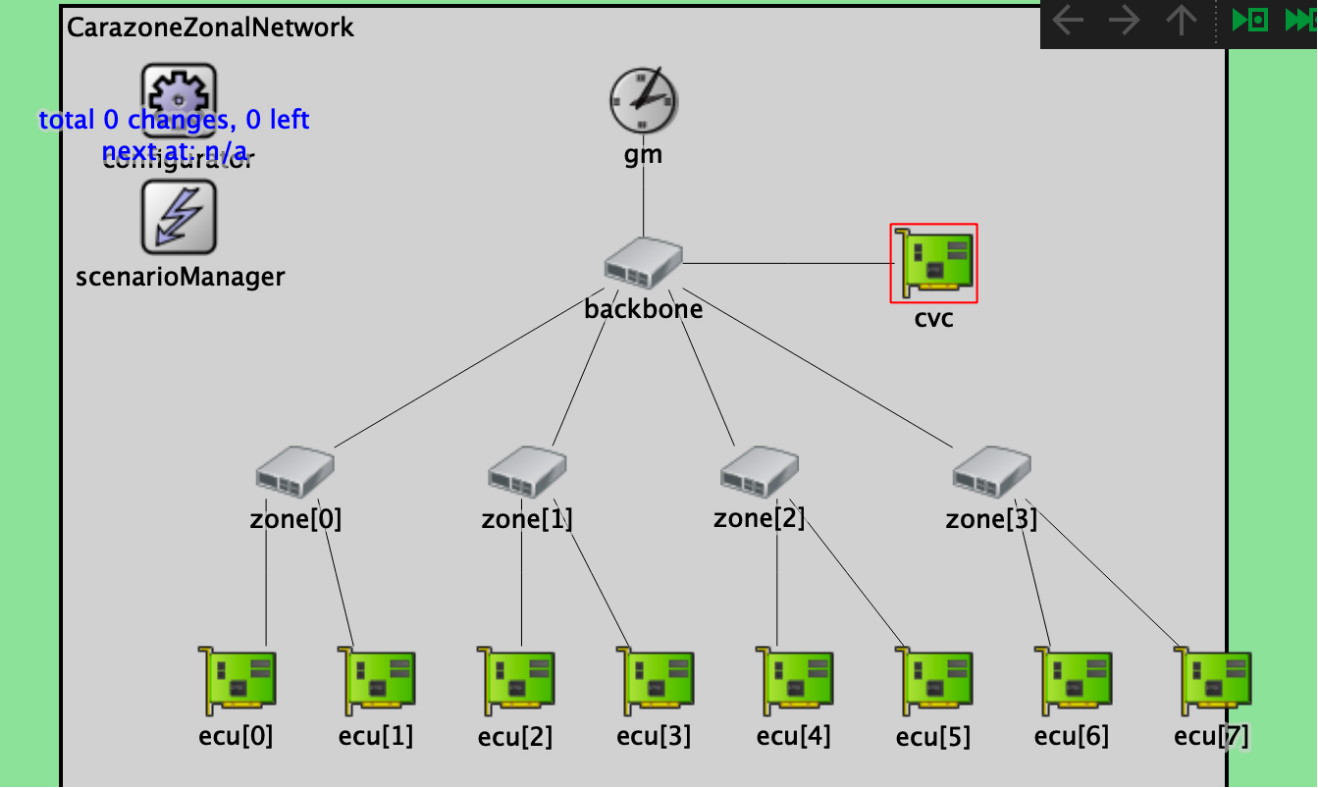
\includegraphics[width=0.95\textwidth]{basictopology.png}
\caption[Implemented four-zone tree topology]{Implemented zonal topology: grandmaster, backbone switch, four zone
controllers, eight endpoint ECUs and the central vehicle compute node.}
\label{fig:topology}
\end{figure}

The implemented topology comprises a grandmaster clock source, a backbone switch,
four zone controllers, eight endpoint ECUs (two per zone), and a central vehicle
compute node attached to the backbone. A configurator and a scenario manager handle
address assignment and timed attack events respectively. All time-aware nodes
participate in a single gPTP domain rooted at the grandmaster, giving a
synchronisation tree of depth three in which the four zone controllers are siblings.

\section{Completed Features / Module}
\begin{itemize}
  \item M1 Zonal Topology Simulation: complete
  \item M2 Attack Injection and Dataset: complete for three attack configurations
  \item M3 Feature Extraction Layer: complete, with DEF-01 open
\end{itemize}

\section{Technical Implementation Details}
\label{sec:technical-details}

\textbf{Environment.} OMNeT++ 6.4.0 with INET 4.7.0~\cite{inettsn}, on macOS (Apple Silicon).
The linked INET version is 4.7.0, which is the version whose
\texttt{driftRate} parameter is not declared \texttt{@mutable}. That property is the
reason the drift attack cannot be activated part-way through a run, and therefore the
reason the drift result in Section~\ref{sec:edge-cases} is reported as a limitation of the framework
rather than a finding about drift detectability.

\textbf{Key files.}
\begin{itemize}
  \item \texttt{CarazoneZonalNetwork.ned}: topology declaration: node types,
        links, and the submodule structure of the zonal network.
  \item \texttt{omnetpp.ini}: scenario configurations. Four named configurations
        are defined: \texttt{Benign}, \texttt{DelayAttack}, \texttt{DriftAttack} and
        \texttt{SyncStarvation}, together with clock drift parameters, gPTP settings
        and seed control.
  \item \texttt{carazone}: the built simulation executable.
  \item \texttt{extract\_features.py}: the feature extraction pipeline.
\end{itemize}

\textbf{Execution.} Scenarios are executed headlessly, selecting a configuration by
name:
\begin{verbatim}
./carazone -u Cmdenv -c Benign
./carazone -u Cmdenv -c DelayAttack
./carazone -u Cmdenv -c DriftAttack
./carazone -u Cmdenv -c SyncStarvation
\end{verbatim}
The graphical environment is used for topology inspection and single-run tracing:
\begin{verbatim}
./carazone -u Qtenv -c Benign -r 0
\end{verbatim}

\textbf{Feature extraction.} Extraction is invoked over a results directory:
\begin{verbatim}
python3 extract_features.py --results ../simulations/results --out features.csv
\end{verbatim}
Window length, stride and simulation limit are command-line parameters with defaults
of 0.25\,s, 0.125\,s and 10\,s respectively. The default window is twice the gPTP
synchronisation interval, so every window is expected to contain at least two
correction events under normal operation. The stride is half the window length,
giving 50\% overlap between consecutive windows. Dependencies are \texttt{pandas},
\texttt{numpy}, and \texttt{opp\_scavetool} from the OMNeT++ distribution on
\texttt{PATH}.

\textbf{Extraction pipeline.} The script proceeds in five stages:

\begin{enumerate}
  \item \texttt{run\_scavetool()} invokes \texttt{opp\_scavetool export -F CSV-R} over
        all \texttt{.vec} files in the results directory, producing one intermediate
        CSV. No scavetool filter expression is applied: match-expression syntax varies
        between tool versions and a rejected expression aborts the export, so the
        pipeline exports everything and filters in pandas. This trades a larger
        intermediate file for version robustness.
  \item \texttt{load\_export()} splits the export into a vector frame and a run-metadata
        frame. Vectors are filtered to names beginning \texttt{timeChanged}, excluding
        modules containing \texttt{underlyingClock} so that each node contributes its
        gPTP-corrected clock rather than its free-running oscillator. Run attributes
        and iteration variables are collected per run, which is how the configuration
        name and the victim zone are recovered.
  \item \texttt{node\_of()} and \texttt{zone\_of()} map a module path to a node and a
        node to a zone. A regular expression matches the node types
        \texttt{gm}, \texttt{cvc}, \texttt{backbone}, \texttt{zone[$i$]} and
        \texttt{ecu[$j$]}. Zone controllers map to their own index; ECUs map by integer
        division by \texttt{ECUS\_PER\_ZONE}. Nodes with no zone (grandmaster,
        backbone and central vehicle compute) are excluded, since they are not
        federated clients.
  \item \texttt{window\_features()} computes eight statistics per node per window. The
        zero-event case returns an explicit record with \texttt{n\_events = 0} rather
        than being discarded, because an empty window is itself the signature of
        synchronisation starvation. Offset is computed as \texttt{v - t} on the recorded
        series, giving error against the ideal timeline.
  \item \texttt{build()} iterates runs, then zones, then windows. For each window it
        computes per-node features, isolates the zone controller's own vector as the
        \texttt{ctrl\_} features, and aggregates mean and standard deviation across all
        nodes in the zone as the \texttt{zone\_} features. Labelling is delegated to
        \texttt{label\_for()}.
\end{enumerate}

\textbf{Labelling logic.} \texttt{label\_for(config, target\_zone, zone, w\_start)}
returns the benign class unless three conditions hold simultaneously: the run
configuration is an attack configuration; the zone under evaluation is the run's
designated victim zone, read from run metadata; and the attack is active over the
window, meaning either the window begins at or after \texttt{ATTACK\_START} or the
configuration is in \texttt{ALWAYS\_ON\_CONFIGS}. A bystander zone in an attack run is
therefore labelled benign, which is what makes zone attribution a learnable target.

\section{Algorithms and Technical Decisions}
\label{sec:algorithms}

\textbf{Windowing.} Raw per-node clock series are segmented into fixed-size
observation windows. The window size is a single global design parameter applied
consistently across all features so that one aligned feature vector is produced per
window per zone.

\textbf{Two-level feature construction.} Each window yields both the zone controller's
own statistics (\texttt{ctrl\_}) and the distribution of those statistics across all
nodes within the zone (\texttt{zone\_mean\_}, \texttt{zone\_std\_}). The controller is
the node that would host the detector in deployment, so its own view is preserved
separately; the within-zone spread captures whether a perturbation affects the
controller alone or the whole zone.

\textbf{Overlapping windows and split granularity.} The stride is half the window
length, so consecutive windows share half their samples. Adjacent windows are therefore
strongly correlated, and a random window-level train/test split would leak information
across the boundary. Splits are consequently formed at run and seed granularity
(integrity rule R3).

\textbf{Planned: cross-zone residual.} The implemented features are all computed within
a single zone. The design intent is that the discriminating feature is a residual
\emph{between} zones, taking a zone's controller offset minus the median across its
siblings in the synchronisation tree, because that is the quantity a generic traffic-feature
detector cannot construct. Computing it requires the observation window to be the outer
loop so that all zones are available simultaneously, which is a restructuring of
\texttt{build()} scheduled in Iteration~03.

\textbf{Consequence for attack coverage.} A sibling residual cancels common-mode
perturbation by construction, and is therefore insensitive to any effect that moves the
whole synchronisation tree together, including compromise at the grandmaster. This is
a structural property rather than a tuning deficiency, and it bounds the detection claim
to link-local timing integrity (Sections~\ref{sec:technical-challenges} and~\ref{sec:edge-cases}).

\section{Tools, Frameworks and Technologies}

\begin{longtable}{p{0.26\textwidth} p{0.16\textwidth} p{0.5\textwidth}}
\toprule
\textbf{Tool} & \textbf{Version} & \textbf{Purpose} \\
\midrule
\endhead
OMNeT++ & 6.4.0 & Discrete-event simulation kernel; Cmdenv for batch runs, Qtenv for
inspection \\
INET~\cite{inettsn} & 4.7.0 & TSN and gPTP protocol models, clock drift modelling \\
Python & 3.x & Feature extraction, dataset construction \\
Flower & not yet adopted & Federated learning framework; selected for Iteration~03, not yet introduced into the build \\
\bottomrule
\end{longtable}

\section{Demonstration Evidence}
\label{sec:demo-evidence}

\begin{figure}[htbp]
\centering
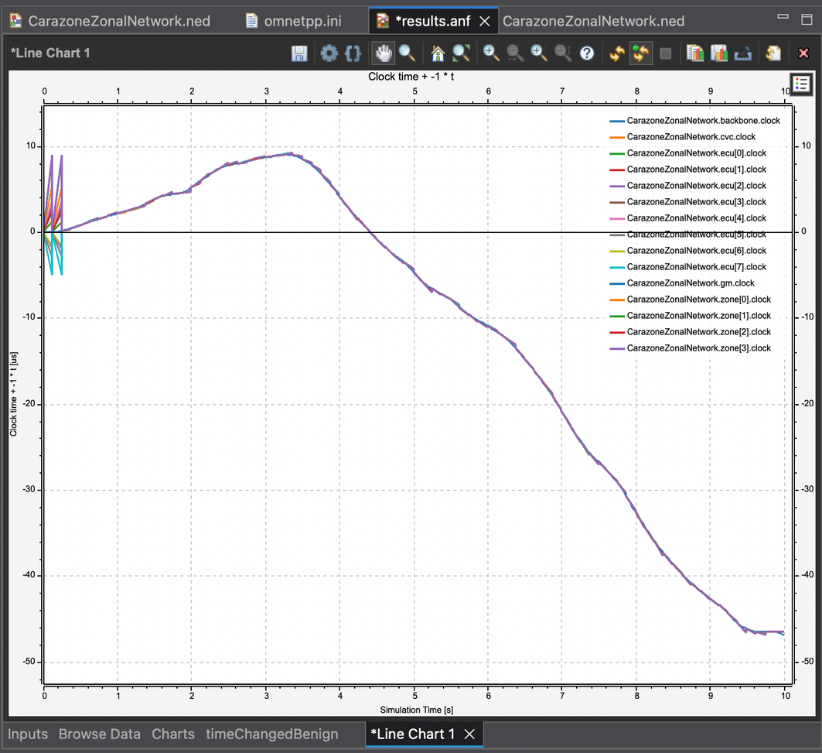
\includegraphics[width=0.92\textwidth]{benign.png}
\caption[Clock offset, benign run]{Clock offset against simulation time, benign run. All fourteen clocks
follow a single common trajectory; the individual traces are not separable at this
scale, which is the expected behaviour of a converged gPTP domain. The transient
before approximately $t = 0.5$~s is the synchronisation servo converging from its
initial state. That transient is the benign population discussed in
Section~\ref{sec:edge-cases}: it produces larger offset excursions than the attack does, which is why
a fixed threshold on offset alone cannot separate the two.}
\label{fig:offset-benign}
\end{figure}

\begin{figure}[htbp]
\centering
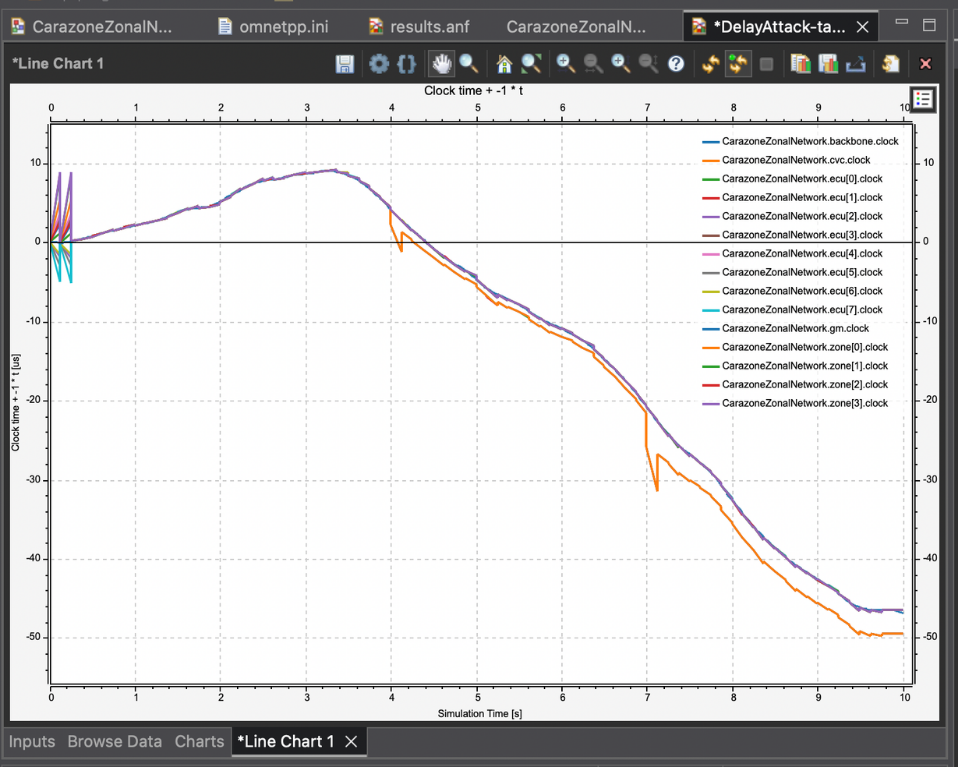
\includegraphics[width=0.92\textwidth]{attack.png}
\caption[Clock offset, delay attack on zone 0]{Clock offset against simulation time, delay attack on zone~0. The targeted
zone controller (orange) separates from the common trajectory at $t = 4$~s, the
attack onset, with a second visible step at $t = 7$~s; every other clock continues
to track the group. The attack is visible only as a disagreement between one zone
and its siblings, not as an absolute fault in the victim's own clock, which is the
observation the cross-zone sibling residual is built to capture
(Section~\ref{sec:algorithms}).}
\label{fig:offset-attack}
\end{figure}

Read together, Figures~\ref{fig:offset-benign} and~\ref{fig:offset-attack} are the
empirical basis of the sibling residual feature. In the benign run every clock
follows one trajectory. In the attacked run the targeted branch departs from that
trajectory at the attack onset while the siblings continue to track one another.
The quantity that changes between the two figures is not the victim's offset in
absolute terms, which continues to follow the same broad shape, but its
\emph{disagreement} with the zones beside it. That is precisely the quantity the
residual measures, and it is why a feature computed inside a single zone cannot see
this attack while a cross-zone comparison can.

\section{Iteration Outcome}
Iterations 01 and 02 met their exit criteria. The simulation produces repeatable,
seeded attack effects; the extraction pipeline produces a labelled dataset. One
defect (DEF-01) and one design limitation (zone symmetry) were identified and are
scheduled for correction before Iteration~03 modelling work begins.

% ============================================================
\chapter{Testing and Early Validation}
\label{ch:testing}
% ============================================================

\section{Testing Strategy}
\label{sec:testing-strategy}
Testing at this stage targets the data generation path rather than the detection
model, on the principle that model results obtained from an unverified dataset are
uninterpretable. Three levels are applied: component checks on extraction logic,
integration checks on the simulation-to-dataset path, and empirical validation that
injected attacks produce the theoretically expected signature.

\section{Test Levels and Techniques}
\label{sec:testing-levels}
\begin{itemize}
  \item \textbf{Component.} Assertions within the extraction pipeline on window
        counts, absence of missing values, and per-zone label distribution.
  \item \textbf{Integration.} End-to-end execution from configuration to dataset,
        verifying row counts and schema conformance.
  \item \textbf{Empirical validation.} Comparison of observed attack signatures
        against the expected theoretical effect, across multiple seeds.
  \item \textbf{Reproducibility.} Repeated execution with identical seeds, comparing
        generated structure and labels.
\end{itemize}

\section{Test Cases}
\label{sec:test-cases}

\begin{longtable}{p{0.07\textwidth} p{0.3\textwidth} p{0.3\textwidth} p{0.25\textwidth}}
\caption{Test cases executed at the mid-report stage}\\
\toprule
\textbf{ID} & \textbf{Objective} & \textbf{Expected} & \textbf{Result} \\
\midrule
\endfirsthead
\toprule
\textbf{ID} & \textbf{Objective} & \textbf{Expected} & \textbf{Result} \\
\midrule
\endhead
TC-01 & Topology instantiates with all declared nodes & All nodes present and linked &
Pass \\
TC-02 & gPTP synchronises all time-aware nodes & Node clocks track a common trajectory
under benign operation & Pass \\
TC-03 & Seeded reproducibility & Identical seed reproduces identical structure and labels &
Pass \\
TC-04 & Delay attack produces measurable deviation & Targeted branch diverges from
siblings during the attack interval & Pass \\
TC-05 & Drift attack produces zone-localisable deviation & Targeted zone diverges from
siblings & \textbf{Not realisable; see Section~\ref{sec:edge-cases}} \\
TC-06 & Extraction produces expected window count & Windows $=$ runs $\times$ zones
$\times$ windows-per-run $= 15 \times 4 \times 79$ & Pass (4{,}740) \\
TC-07 & Zero-event windows are retained, not dropped & Window with no clock event
yields a record with \texttt{n\_events}$=0$ & Pass \\
TC-08 & Attack labels attributed to victim zone only & In an attack run targeting zone
$z$, only zone $z$ carries the attack label & Pass (see Section~\ref{sec:test-results}) \\
TC-09 & Dataset conforms to the documented schema & Column names, order and types match
Table~\ref{tab:schema} & Pass (after schema amendment; see Section~\ref{sec:defects}) \\
\bottomrule
\end{longtable}

\section{Test Results}
\label{sec:test-results}

Fifteen seeded runs produced 225 recorded vectors, from which the extraction pipeline
generated 4{,}740 labelled feature windows.

\begin{longtable}{p{0.14\textwidth} r r r}
\caption{Label distribution by zone}\label{tab:labels}\\
\toprule
\textbf{Zone} & \textbf{Benign} & \textbf{Attack} & \textbf{Total} \\
\midrule
\endfirsthead
\toprule
\textbf{Zone} & \textbf{Benign} & \textbf{Attack} & \textbf{Total} \\
\midrule
\endhead
Zone 0 & 1{,}044 & 141 & 1{,}185 \\
Zone 1 & 1{,}044 & 141 & 1{,}185 \\
Zone 2 & 1{,}044 & 141 & 1{,}185 \\
Zone 3 & 1{,}044 & 141 & 1{,}185 \\
\midrule
\textbf{Total} & \textbf{4{,}176} & \textbf{564} & \textbf{4{,}740} \\
\bottomrule
\end{longtable}

\textbf{Derivation of the distribution.} With a window of 0.25\,s, a stride of
0.125\,s and a simulation limit of 10\,s, each run yields 79 windows per zone. The
observed 1{,}185 windows per zone therefore correspond to exactly 15 runs. Attacks
begin at $t=4.0$\,s, so 47 of the 79 windows per run fall within the attack interval.
The observed 141 attack-labelled windows per zone correspond to $3 \times 47$, that is,
each zone is the designated victim in exactly three runs. The run set is accordingly
3 benign runs and 12 delay-attack runs, covering four victim zones at three seeds each,
giving $12 \times 47 = 564$ attack windows in total.

\textbf{Victim rotation.} Rotating the victim zone across runs is a deliberate design
choice. Had a single zone been targeted throughout, zone identity would correlate
perfectly with the label and any classifier could reach high accuracy by learning zone
index alone. Because every zone appears as victim in three runs and as bystander in
nine, zone identity carries no label information and attribution must be learned from
the timing features.

\textbf{Class imbalance.} The benign-to-attack ratio is approximately $7.4{:}1$.
Accuracy is therefore excluded as a reported measure; evaluation uses per-class
precision, recall and F1, macro-F1, and detection rate at a fixed false-positive rate.

\section{Acceptance Testing / Validation}
\label{sec:acceptance-validation}

Acceptance checks defined in Section~\ref{sec:acceptance-criteria} have been exercised for FR-01 through FR-09.
Checks for FR-10 to FR-15 and NFR-08 require the federation and
monitoring-interference work scheduled for Iteration~04 and are reported as planned in
Section~\ref{sec:validation-plan}.

Success criterion SC-2, that protocol-native features outperform features computable
without knowledge of network structure, has been tested centrally ahead of schedule,
because it is the premise on which the federated work depends and a null result would
have required repositioning the project. The experiment is a feature ablation with
identical models and identical splits across three feature sets:

\begin{itemize}
  \item \textbf{within\_zone} (24 features): all \texttt{ctrl\_} and \texttt{zone\_}
        statistics. These describe one zone's clock behaviour in isolation and require
        no knowledge of the synchronisation tree. This is the control arm.
  \item \textbf{residual} (2 features): the cross-zone sibling residuals only.
  \item \textbf{combined} (26 features): both.
\end{itemize}

Splits are formed by holding out whole runs, stratified so that both benign and attack
runs appear on each side, and averaged over five resplits. Window-level splitting is
not used: the extraction stride is half the window length, so adjacent windows share
half their samples and a random split would place near-duplicates on both sides.

\begin{longtable}{p{0.22\textwidth} p{0.14\textwidth} r r r}
\caption{Feature ablation, macro-F1 averaged over five run-level splits}
\label{tab:ablation}\\
\toprule
\textbf{Feature set} & \textbf{Model} & \textbf{Macro-F1} & \textbf{Attack recall} &
\textbf{Latency (windows)} \\
\midrule
\endfirsthead
\toprule
\textbf{Feature set} & \textbf{Model} & \textbf{Macro-F1} & \textbf{Attack recall} &
\textbf{Latency (windows)} \\
\midrule
\endhead
Majority-class floor & n/a & 0.468 & n/a & n/a \\
\midrule
within\_zone  & logistic reg. & 0.500 & 0.419 & 11.6 \\
within\_zone  & MLP           & 0.481 & 0.013 & 25.0 \\
within\_zone  & random forest & 0.536 & 0.259 & 12.7 \\
\midrule
residual      & logistic reg. & 0.951 & 1.000 & 2.0 \\
residual      & MLP           & 0.968 & 0.993 & 2.0 \\
residual      & random forest & \textbf{0.984} & 0.994 & 2.5 \\
\midrule
combined      & logistic reg. & 0.975 & 0.997 & 2.0 \\
combined      & MLP           & 0.966 & 0.919 & 2.0 \\
combined      & random forest & 0.969 & 0.930 & 2.0 \\
\bottomrule
\end{longtable}

\textbf{Result 1: within-zone features do not detect this attack.} All three
within-zone arms fall between 0.481 and 0.536 macro-F1 against a majority-class floor
of 0.468. The MLP arm attains 0.013 attack recall, that is, it classifies almost every
window as benign. Features describing a single zone's clock in isolation carry
essentially no information about this attack, because the attack does not make the
victim's clock behave abnormally in absolute terms; it makes the victim disagree with
its siblings.

\textbf{Result 2: two cross-zone features are sufficient.} The residual arm reaches
0.951--0.984 macro-F1 using two columns. The gain over the control arm is $+0.475$,
$+0.485$ and $+0.433$ macro-F1 for logistic regression, MLP and random forest
respectively. SC-2 is therefore met, and met by a margin that does not depend on model
choice.

\textbf{Result 3: the larger feature set is not the better one.} For the MLP and random
forest, the residual arm alone outperforms the combined arm (0.984 against 0.969 for
random forest). The 24 within-zone features dilute rather than augment the signal. This
is relevant to NFR-05: a detector intended to run on a resource-constrained zone
controller benefits from a deliberately small feature set, and the evidence here is that
the small set is also the more accurate one.

\textbf{Result 4: both residual features are necessary.} That logistic regression, a
linear decision boundary, reaches 0.951 macro-F1 on two features implies that the
classes are linearly separable in the two-dimensional residual space. They are not
separable in the offset dimension alone, as Section~\ref{sec:edge-cases} shows. The drift-slope residual
is therefore load-bearing despite appearing weak when summarised univariately, and the
mechanism by which it contributes is recorded in Section~\ref{sec:edge-cases}.

\textbf{Detection latency.} With a confirmation requirement of three consecutive
anomalous windows, detection fires two windows after attack onset for every
residual-based arm. At a stride of 0.125\,s and a synchronisation interval of
0.125\,s, that is two synchronisation intervals, which is the minimum achievable under
a three-window confirmation rule. The within-zone arms require 11.6 to 25.0 windows,
the upper value indicating that detection frequently does not occur at all within the
run.

\textbf{Error structure.} For the combined random-forest arm the confusion matrix over
a held-out split is $\left(\begin{smallmatrix}1389 & 3\\ 0 & 188\end{smallmatrix}\right)$
(rows true, columns predicted): no attack window is missed, and three benign windows
are misclassified. Logistic regression shows the same structure with nine false
positives and no false negatives. The error is therefore one-sided towards false alarm
rather than missed detection, which is the preferable direction for a safety-relevant
monitor, though it makes the false-alarm rate the quantity requiring most attention at
deployment scale (Section~\ref{sec:validation-plan}).

\section{Edge and Failure Cases}
\label{sec:edge-cases}

\textbf{Negative result: oscillator drift manipulation is not realisable as a runtime
attack under the current simulation framework.} An attack was designed in which the
scenario manager would alter the local oscillator drift rate of a victim node partway
through a run, producing a zone-localised divergence from the remaining zones.

The attack could not be implemented in that form. The clock module's drift-rate
parameter is not declared mutable in the INET version in use, so the scenario manager
cannot modify it at simulation time. The implementation therefore applies the
manipulated drift rate from $t=0$, which is why the \texttt{DriftAttack} configuration
appears in the extraction script's \texttt{ALWAYS\_ON\_CONFIGS} set rather than being
gated on the attack start time.

Applied from $t=0$, the manipulation is not an attack in any meaningful sense: it is a
node whose oscillator runs at a different constant rate for the whole simulation, which, in the clock-offset dimension measured here, is indistinguishable from legitimate
component variation and which the gPTP servo is specifically designed to compensate. The observed network-wide behaviour is the protocol
operating correctly, not a detection failure.

Three consequences are carried forward. First, the finding is a statement about attack
realisability under this framework, not about the detectability of drift attacks in
general; the stronger claim is not supported by this experiment and is not made.
Second, drift is removed as a committed target for the cross-zone offset residual,
reducing the committed attack set to delay injection and synchronisation starvation; a
separate candidate signal for constant drift is described below. Third, if a runtime drift attack
is required in FYP-2, it must be realised by a different mechanism, for example by
subclassing the clock module to expose a mutable rate, or by post-processing the
recorded trace, and the cost of that work is weighed against the alternative of
deepening the evaluation of the two realisable attack classes.

\textbf{Update from the ring topology.} Constant drift applied from $t=0$ was later
re-run on the five-zone ring with the gPTP correction signals recorded
(Section~\ref{sec:ring-results}). The clock offset still hides it, but
\texttt{gmRateRatio} moves from about 0.99999 to about 0.99800 at 2000~ppm, so the signal
that is absent from the offset dimension is present in the rate-ratio dimension. This does
not change the realisability finding above, since a runtime drift attack remains
unrealisable, and it leaves the committed attack set unchanged pending extraction of
rate-ratio features.

\textbf{Negative result: no fixed threshold separates attack from benign behaviour.}
Two tuned thresholds on the absolute sibling offset residual were evaluated as
non-learned baselines. The first was set to the largest residual observed on benign
training windows, which by construction admits all benign training behaviour. The
second was set to the 99.5th percentile of that distribution, discarding the extreme
tail. Both attained zero recall on held-out data: every attack window fell below both
thresholds.

The cause is the gPTP convergence transient. Table~\ref{tab:populations} separates
benign windows by simulation time.

\begin{longtable}{p{0.34\textwidth} r r}
\caption{Absolute sibling offset residual by population}\label{tab:populations}\\
\toprule
\textbf{Population} & \textbf{Median (s)} & \textbf{Maximum (s)} \\
\midrule
\endfirsthead
\toprule
\textbf{Population} & \textbf{Median (s)} & \textbf{Maximum (s)} \\
\midrule
\endhead
Benign, $t < 1$\,s (convergence) & $1.00\times10^{-8}$ & $1.51\times10^{-5}$ \\
Benign, $t \geq 1$\,s (steady state) & $4.83\times10^{-9}$ & $1.81\times10^{-6}$ \\
Delay attack & $2.19\times10^{-6}$ & $5.66\times10^{-6}$ \\
\bottomrule
\end{longtable}

Before the clock servos lock, zones disagree with one another by more than any injected
attack subsequently moves them: the convergence maximum exceeds the largest attack
residual by a factor of 2.7. Those early windows are legitimately benign, so any
threshold admitting all benign behaviour must sit above the startup excursion and is
consequently blind to the attack in steady state.

The percentile variant fails for a quantitative reason worth stating. Windows beginning
before $t = 1$\,s constitute approximately 11\% of all benign windows, so any percentile
above roughly the 89th remains inside the convergence population. The failure is
therefore not an artefact of a poorly chosen cut-off: no percentile-based threshold
succeeds while the convergence transient is part of the benign class.

This is a stronger justification for the learned detector than the ablation alone
provides. The ablation establishes which features carry the signal; this result
establishes that the signal is not separable by a single decision boundary on the
offset residual, because the benign class is not unimodal; it is a mixture of a
steady-state population and a convergence population, and the attack lies between them
in magnitude.

\textbf{Why two residual features are required.} The second residual feature,
computed on the drift slope rather than the mean offset, is a weak discriminator when
measured alone: the ratio of its median under attack to its median under benign
operation is approximately 2.0, against 438 for the offset residual. It is nevertheless
not redundant. The residual feature set contains only these two columns, and logistic
regression, a linear decision boundary, attains 0.951 macro-F1 on them
(Table~\ref{tab:ablation}). A linear boundary can only achieve this if the three
populations are linearly separable in the two-dimensional residual space, which they
are not in the offset dimension alone.

The mechanism is that the two populations the offset residual confuses are distinguished
by the slope. During convergence the servos are actively correcting, so successive
offsets change rapidly and the slope residual is large. The delay attack introduces a
steady asymmetry, so the victim's offset departs from its siblings along a near-constant
gradient and the slope residual remains small. The slope residual is therefore not a
second detector of the attack; it is the feature that excludes the benign convergence
population from the region of offset-residual space that the attack occupies. This is
the reason a univariate summary understates its contribution, and it is recorded here
because the measurement that reveals it, a linear model succeeding on two features,
is easily mistaken for an unimportant result.

The practical consequence for FYP-2 is that the attack-intensity sweep (Section~\ref{sec:validation-plan})
must report the benign envelope, separated into convergence and steady-state
populations, alongside detection rate rather than reporting detection rate alone.

\textbf{Pending: grandmaster-level perturbation.} A separate structural limitation
follows from the planned sibling-residual feature rather than from any implemented
result. A residual between siblings cancels common-mode perturbation by construction,
so it cannot detect an effect that moves the entire synchronisation tree together,
including compromise at the time source itself. This bounds the detection claim to
link-local timing integrity. Detecting time-source compromise would require an
independent reference such as local oscillator holdover comparison or a second
synchronisation domain, and is out of scope.

\textbf{Pending edge cases.} Attack intensities approaching the benign drift envelope,
unseen seeds, and coordinator or model unavailability are scheduled for Iteration~04
(Section~\ref{sec:validation-plan}).

\section{Defects and Corrective Actions}
\label{sec:defects}

\textbf{DEF-04. Schema drift between the documented column contract and the emitted
dataset.} Test TC-09 compared the columns of \texttt{features.csv} against the
contract in Table~\ref{tab:schema} and found three columns present in the data but
absent from the contract: \texttt{target\_zone}, and the two
\texttt{sibling\_n\_\{f\}} counts emitted alongside each residual.
\emph{Consequence:} a reader implementing against the documented contract would not
have anticipated them, and \texttt{target\_zone} in particular is equivalent to the
label, so an implementer unaware of it could leak ground truth into a model.
\emph{Recovery:} the contract in Table~\ref{tab:schema} was corrected to document all
three, and the leakage risk is additionally guarded by an automated test asserting
that no identifier column reaches any feature set (Appendix~\ref{app:test-cases}). Status:
\textbf{closed}.

\begin{longtable}{p{0.08\textwidth} p{0.3\textwidth} p{0.26\textwidth} p{0.28\textwidth}}
\caption{Defect register}\\
\toprule
\textbf{ID} & \textbf{Description} & \textbf{Impact} & \textbf{Corrective action} \\
\midrule
\endfirsthead
\toprule
\textbf{ID} & \textbf{Description} & \textbf{Impact} & \textbf{Corrective action} \\
\midrule
\endhead
DEF-01 & The feature set contained no cross-zone comparison; all features were
computed within a single zone. &
The features were not structurally exclusive to a deterministic network, so SC-2 could
not be tested. &
\texttt{build()} restructured to iterate window-then-zone, and two sibling residual
features emitted. Verified by the ablation in Section~\ref{sec:acceptance-validation}: within-zone features reach
0.48--0.54 macro-F1, residual features 0.95--0.98. Status: \textbf{closed}. \\
\addlinespace
DEF-02 & All four zones of the Iteration~1 topology carry identical traffic profiles
and produce identical window counts. &
Federated, centralized and local-only training would converge to equivalent models,
making the federated comparison (SC-4) null by construction. &
The five-zone reference topology (Section~\ref{sec:ref-topology}) introduces structural asymmetry: three
to seven ECUs per zone, distinct traffic classes by zone function, and gPTP delay that
grows with hop distance from the grandmaster. Status: \textbf{partially addressed}.
Designed but not measured; closes when per-zone divergence is quantified and
differentiated traffic profiles are running. \\
\addlinespace
DEF-03 & The attack start time is hard-coded in the extraction script as a module
constant and must be kept consistent with the simulation configuration by hand. &
A change to the attack schedule in the simulation that is not mirrored in the extraction
script would mislabel the dataset silently. &
Read the attack start time from run metadata rather than from a constant, and add an
assertion that fails extraction when the two disagree. Status: open, low effort. \\
\bottomrule
\end{longtable}

\section{Current Validation Status}

The data generation path is validated for one attack class and found defective in one
respect. The detection and federation paths are unvalidated because they are
unimplemented. No detection performance figures are claimed at this stage, and none
should be inferred from the dataset statistics reported above. The attack simulations on
the five-zone ring (Section~\ref{sec:ring-results}) are single-run observations of candidate
signals; they have not been extracted into the dataset, and no detection performance is
claimed from them.

% ============================================================
\chapter{Project Management and Development Evidence}
% ============================================================

\section{Work Completed}
Zonal TSN topology with gPTP synchronisation; attack injection harness with three
instrumented configurations; 15 seeded simulation runs producing 225 recorded
vectors; feature extraction pipeline producing 4{,}740 labelled windows; empirical
validation of delay-attack signature; identification and characterisation of one
negative result and two defects; literature review and departmental-repository gap
comparison; operator-facing alert surface as a presentation mock-up.

\section{Work Remaining}
Correction of DEF-01 and DEF-02; centralized detection model and the
protocol-native-versus-generic-feature comparison; federated training pipeline with
local-only, centralized and FedAvg arms; zone attribution evaluation; detection
latency measurement; monitoring-interference measurement (NFR-08); alert surface
driven by real model output; rule-based fallback.

\section{Individual Responsibilities}
Responsibilities follow the allocation in Table~\ref{tab:workbreakdown}
(Section~\ref{sec:workbreakdown}). The split is by area rather than by task, so that each member owns a
coherent part of the system end to end and can explain it independently. Adeena Zaib
owns the simulation and data-generation path: the OMNeT++/INET topology, the attack
scenarios, and the per-zone dataset packaging that feeds the federated clients.
Khaula Bilqees owns the TSN signal instrumentation, the labelling scheme, and the
federated client and server implementation.

\section{Contribution of Each Team Member}
The artefacts produced in this reporting period are listed below against their owner.
Each is verifiable against the commit history in Appendix~\ref{app:repository} rather than asserted here.

\textbf{Khaula Bilqees.} The OMNeT++/INET zonal topology and its scenario
configurations, committed as \texttt{8b765f6}; and the subsequent topology and
configuration revisions in \texttt{31cb803} and \texttt{f009ac6}.

\textbf{Adeena Zaib.} The initial proof of concept (\texttt{0506e63}); the feature
extraction pipeline including the window construction, the labelling rule and the
cross-zone sibling residual (\texttt{856beba}); and the continuous integration
workflow with its automated test suite (\texttt{ed4b0f6}, \texttt{2168990}).

The commit record shows seven commits, four from the first author and three from the
second, with both members committing under their own accounts throughout.

\textbf{Divergence from the planned allocation.} Table~\ref{tab:workbreakdown} in
Section~\ref{sec:workbreakdown} allocates the topology to the first author and the signal instrumentation
to the second. In practice these two areas were exchanged during Iteration~1: the
topology was implemented by the second author and the extraction pipeline by the
first. The allocation of the remaining areas is unchanged, and the federated client
and server implementation scheduled for Iteration~03 remains with the second author.
This is recorded rather than quietly corrected, because the commit history is the
evidence for this section and it should agree with the text.

\section{Repository and Version Control Evidence}
\label{sec:repository}
The project is held in a Git repository with both members committing under their own
accounts. Continuous integration is configured through GitHub Actions: a workflow runs
on every push and executes the automated test suite described in Section~\ref{sec:testing-levels}, so a
change that breaks the feature extraction or training pipeline is caught at the point
it is pushed rather than at the next manual run.

The repository is at \url{https://github.com/AdeenaZaib/VROOM}. The commit log and
the per-member commit counts are reproduced in Appendix~\ref{app:repository}.

\begin{figure}[htbp]
\centering
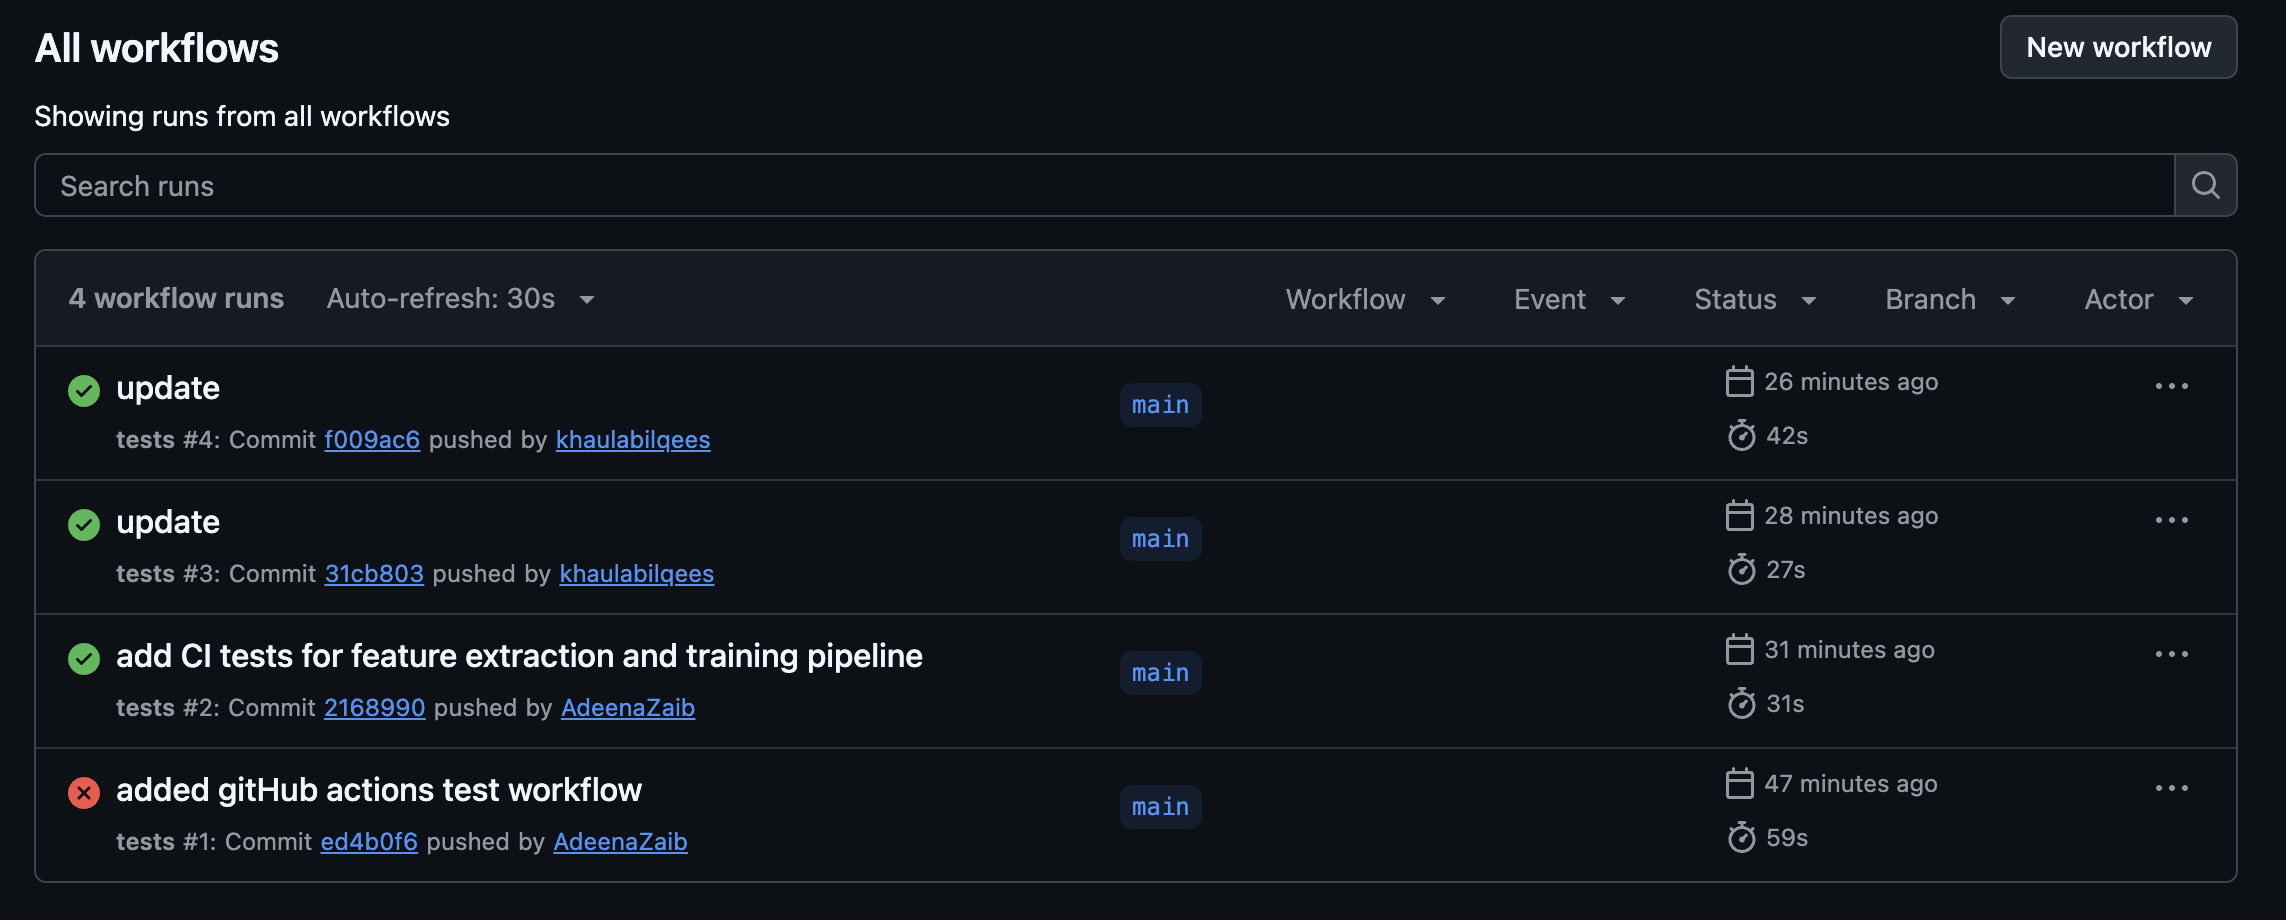
\includegraphics[width=0.95\textwidth]{workflow.png}
\caption[GitHub Actions run history]{GitHub Actions run history. Each run is tied to a commit and to the member
who pushed it, which is the per-member development evidence this section reports.
Run \#1 failed and the following runs pass, which records a real correction rather
than a repository created immediately before submission.}
\label{fig:ci}
\end{figure}

Two properties of this history are worth stating explicitly, because they are what
the evidence is for. First, the pushes are distributed across both members:
runs \#1 and \#2 were pushed by the first member and runs \#3 and \#4 by the
second, so the contribution record is visible in the tooling rather than asserted in
this document. Second, the first run failed and subsequent runs pass. That sequence
is retained deliberately: it shows the pipeline being established and corrected during
the reporting period.

\section{Milestones and Commit Evidence}
The automated suite is itself the milestone evidence for modules M2 and M3. It
contains fourteen tests, of which three are dataset invariants that run only when
\texttt{features.csv} is present and are therefore exercising the real extracted
dataset rather than synthetic fixtures. Three of those tests encode the corrections
recorded as defects in Section~\ref{sec:defects}: that attack labels are confined to the target
zone (DEF-01), that the cross-zone residual is not identically zero, and that the
victim zone rotates across runs so that the detector cannot memorise a single zone.

\begin{longtable}{p{0.14\textwidth} p{0.30\textwidth} p{0.46\textwidth}}
\caption{Milestones against the commits that completed them}\label{tab:milestones}\\
\toprule
\textbf{Commit} & \textbf{Milestone} & \textbf{Module and evidence} \\
\midrule
\endfirsthead
\toprule
\textbf{Commit} & \textbf{Milestone} & \textbf{Module and evidence} \\
\midrule
\endhead
\texttt{0506e63} & Proof of concept & Pre-proposal demonstrator \\
\addlinespace
\texttt{8b765f6} & M1 complete: zonal topology simulated &
\texttt{CarazoneZonalNetwork.ned}; Figure~\ref{fig:topology} \\
\addlinespace
\texttt{856beba} & M3 complete: feature extraction, including the cross-zone residual &
\texttt{extract\_features.py}; ablation in Section~\ref{sec:acceptance-validation} \\
\addlinespace
\texttt{ed4b0f6} & Continuous integration established &
First workflow run; failed, and corrected in the next commit \\
\addlinespace
\texttt{2168990} & Automated test suite covering M2 and M3 &
Fourteen tests; three encode the DEF-01 correction (Appendix~\ref{app:test-cases}) \\
\addlinespace
\texttt{31cb803}, \texttt{f009ac6} & Topology and configuration revisions &
Passing workflow runs \#3 and \#4 \\
\bottomrule
\end{longtable}

\section{Tools and Tool-Assisted Development}

\begin{longtable}{p{0.24\textwidth} p{0.3\textwidth} p{0.38\textwidth}}
\caption{Tool and AI-assistance disclosure}\\
\toprule
\textbf{Tool} & \textbf{Used for} & \textbf{Boundary} \\
\midrule
\endfirsthead
\toprule
\textbf{Tool} & \textbf{Used for} & \textbf{Boundary} \\
\midrule
\endhead
OMNeT++ / INET & Simulation framework & Standard open-source components used as
published; the topology, scenario configurations and attack injection logic are the
team's own work \\
\addlinespace
Generative AI assistants & Literature search support, document drafting, code
scaffolding, report structuring and review &
Core detection model design, federated architecture decisions, attack
implementation, simulation configuration, experimental results and their
interpretation are the team's own work. Generated text has been reviewed, verified
against primary sources and rewritten by the authors. No reported result is AI
generated. \\
\bottomrule
\end{longtable}

% [[VERIFY]] Extend this to the exact level of disclosure your department requires,
% and ensure both members can explain any section they did not personally draft.

\section{External Components and Dependencies}
\label{sec:dependencies}

\begin{longtable}{p{0.2\textwidth} p{0.14\textwidth} p{0.2\textwidth} p{0.36\textwidth}}
\toprule
\textbf{Component} & \textbf{Version} & \textbf{Licence} & \textbf{Use} \\
\midrule
\endhead
OMNeT++ & 6.4.0 & Academic Public License & Simulation kernel \\
INET & 4.7.0 & LGPL & TSN, gPTP, clock models \\
Python & 3.x & PSF & Extraction, training \\
Flower & not yet adopted & Apache 2.0 & Federated learning framework; selected for Iteration~03, not yet introduced into the build \\
\bottomrule
\end{longtable}

\section{Risks and Mitigation}

\begin{longtable}{p{0.24\textwidth} p{0.1\textwidth} p{0.28\textwidth} p{0.28\textwidth}}
\caption{Risk register}\\
\toprule
\textbf{Risk} & \textbf{L\,/\,I} & \textbf{Mitigation} & \textbf{Trigger / fallback} \\
\midrule
\endfirsthead
\toprule
\textbf{Risk} & \textbf{L\,/\,I} & \textbf{Mitigation} & \textbf{Trigger / fallback} \\
\midrule
\endhead
Protocol-native features do not outperform generic traffic features &
Med / High &
Run the controlled comparison centrally and early, before federated infrastructure is
built &
If no advantage is demonstrated, report the negative result and reposition the
contribution around federated zone-level detection and attribution \\
\addlinespace
Required internal protocol state is not exposed by the simulation framework &
Med / High &
Verify observability per feature before committing the feature &
Substitute an observable proxy or instrument the module explicitly \\
\addlinespace
FedAvg does not outperform local-only training under non-IID zones &
Med / Med &
Introduce genuine zone heterogeneity; normalise features; report worst-client
performance &
Report as a legitimate finding; FedProx retained as an extension, not a rescue \\
\addlinespace
Feature leakage through adjacent-window splitting &
Med / High &
Split by run and seed, never by window (integrity rule R3) &
Rebuild the dataset and record the change \\
\addlinespace
Scope expansion through additional attacks or models &
High / High &
Protect committed scope; extensions gated on completion of the core path &
Drop schedule-window detection, FedProx and conformal calibration first, in that
order; reduce FRER to a single redundant stream pair before dropping it \\
\addlinespace
Remaining implementation compressed into FYP-2 &
High / High &
Sequence the decision gate first so that a null result is found early &
Reduce to a single attack class with full evaluation rather than several partially
evaluated \\
\bottomrule
\end{longtable}

\section{Security and Privacy Considerations}
All data is synthetic. No personal, vehicle or OEM data is processed. The federated
design transmits model parameters only; raw feature records never leave the client
(NFR-07), which is verified by the acceptance check on FR-13. Attack implementations
are confined to the simulation environment. Secure aggregation, differential privacy
and model-poisoning resistance are outside committed scope and are stated as
limitations rather than claimed properties.

\section{Current Limitations}
\label{sec:limitations}
\begin{enumerate}
  \item Detection results are centralized only; no federated result is claimed.
  \item Zones are currently symmetric, so federated behaviour cannot yet be assessed.
  \item The injected attack is large relative to the benign steady-state envelope; the
        intensity at which detection degrades has not been established.
  \item Oscillator drift manipulation is not realisable as a runtime attack under the
        current framework, reducing the committed attack set to two classes.
  \item Time-aware shaping is not configured, so schedule-conformance features and
        deadline-miss consequences are unavailable.
  \item The approach is insensitive to grandmaster-level compromise by construction.
  \item The static-environment assumption (A1) excludes networks that reconfigure at
        runtime.
  \item Evaluation is simulation-only; attacks are synthetic and no hardware
        validation is performed.
  \item The alert surface is a presentation mock-up and is not yet driven by model
        output.
\end{enumerate}

% ============================================================
\chapter{Remaining FYP Plan}
\label{ch:plan}
% ============================================================

\section{Remaining Scope}
Objectives O4--O6: detection model, federated training and comparative evaluation,
and attributed alerting driven by real model output.

\section{Remaining Modules and Features}
M4 Federated Detection Model; M5 Zone Participation and Aggregation; M6 Alerting and
Presentation; the redundant-topology and IEEE 802.1CB FRER extension to M2 (topology
and attack injection) and M3 (feature extraction); plus corrective work on M2 and M3
(DEF-01, DEF-02).

\section{Remaining Iterations}
\label{sec:remaining-iterations}

\textbf{Iteration 03: Detection and decision gate. Complete.}
The cross-zone sibling residual was added, a centralized detector trained, and the
feature ablation completed. The decision gate is passed: cross-zone features exceed
within-zone features by $+0.43$ to $+0.49$ macro-F1 across three models, so the
federated work proceeds as planned.

\textbf{Iteration 03b: Dataset depth.}
Extract the \texttt{SyncStarvation} configuration to give a genuine multiclass problem.
Sweep the injected attack intensity downwards to establish the detection boundary
against the benign envelope. Introduce differentiated per-zone traffic profiles
(DEF-02).

\textbf{Iteration 03c: Redundant topology and FRER.}
The topology half of this iteration is complete in design: the five-zone ring
(Section~\ref{sec:ref-topology}) is generated and passes its structural checks, including the
single-link-cut partition test that establishes disjoint paths. What remains is to run
the benign baseline on it and record the four behavioural checks listed in
Section~\ref{sec:topology-validation}, then configure IEEE 802.1CB sequence generation at the talkers and
sequence recovery at the listeners for the redundant streams. Implement
stream-redundancy manipulation as a third attack class: selective suppression or
delay of one member of a replicated stream in a single target zone. Add the FRER
feature family to \texttt{extract\_features.py}, namely inter-member arrival skew,
sequence-number deviation between redundant members, and per-member inter-arrival
cadence, together with their cross-zone sibling residuals, computed by the same
window-outer, zone-inner construction already used for the gPTP features. Exit
criterion: the FRER residual features reach macro-F1 $> 0.90$ on the redundancy
attack class while the corresponding within-zone features remain at chance, which
would show the residual principle to be a property of the zonal architecture rather
than of the synchronisation plane alone. This iteration is independent of
Iteration~03b and may run in parallel, since it touches the topology and the feature
extractor rather than the detector. Migrating the gPTP attack configurations from the
four-zone tree to the five-zone ring is a prerequisite for both, and is the point at
which the Chapter~\ref{ch:testing} results are re-established on the reference topology.

\textbf{Iteration 04: Federation and evaluation.}
Federated client/server implementation; local-only, centralized-pooled and FedAvg
arms on identical splits; zone attribution evaluation; detection latency; alert
surface driven by model output; rule-based fallback; monitoring-interference
measurement.

\section{Implementation Plan}
Iteration 03 proceeds in strict order: labelling correction, heterogeneity, third
attack class, control arm, comparison. The ordering is deliberate, because each step is a
precondition for interpreting the next. Iteration 03c runs in parallel on the
topology and extraction path: redundant links, 802.1CB sequence generation and
recovery, redundancy attack injection, then the FRER feature family and its
residuals. Iteration 04 proceeds in order: local-only
baseline, centralized upper bound, FedAvg, then the remaining evaluation dimensions.

\section{Testing and Validation Plan}
\label{sec:validation-plan}

\begin{longtable}{p{0.28\textwidth} p{0.66\textwidth}}
\toprule
\textbf{Evaluation dimension} & \textbf{Metrics} \\
\midrule
\endhead
Detection quality & Per-class precision, recall, F1; macro-F1; confusion matrix;
detection rate at fixed false-positive rate \\
Feature-set comparison & Macro-F1 of protocol-native versus generic traffic features,
identical model and splits, reported across seeds \\
Operational detection & Detection latency in synchronisation intervals; false alarms
per vehicle-hour \\
Attribution & Zone attribution top-1 accuracy, reported separately from detection \\
Federated behaviour & Worst-client macro-F1; centralized-to-FedAvg gap; convergence
rounds; update volume per round \\
Baselines & Fixed threshold on raw offset; CUSUM on sibling residual; LOF (for
comparability with published gPTP work) \\
TSN behaviour & Protected-stream mean and 99th-percentile latency, monitoring enabled
versus disabled (NFR-08) \\
Reproducibility & Results across fixed seeds, held-out attack episodes and held-out
configurations \\
\bottomrule
\end{longtable}

Accuracy is excluded as a headline measure throughout, owing to the class imbalance
reported in Section~\ref{sec:test-results}. Train/test separation is performed at run and seed
granularity (integrity rule R3).

\section{Deployment Plan}
\label{sec:deployment-plan}
The deliverable is a reproducible research and validation environment: pinned
dependencies, documented commands, sample configurations, seeds, and exported
results, executable by a non-author on a clean environment.

Two consumers of detector output are defined. Within the vehicle, the integrity
verdict (class, affected branch, confidence) is the decision input that
fault-tolerant timing mechanisms require in order to fail over or enter holdover; the
relevant standardised machinery provides the failover mechanism but leaves the
domain-quality decision unspecified. Off-vehicle, attributed alerts populate the vSOC
incident queue, where per-vehicle anomalies are triaged against fleet-wide
correlation.

\section{Tentative Timeline}
The project proposal was defended on 11 September 2026 and this mid evaluation falls
in the week of 13 October 2026. The final FYP-1 evaluation is scheduled for December
2026, which is the deadline the sequence below is sized against. The sequence is
ordered by dependency rather than by date. Iterations 03b and
03c are independent of each other and may run in parallel; Iteration 04 depends on
both, because the federated comparison is meaningless until the clients differ
(03b) and incomplete until the second attack family exists (03c).

\begin{longtable}{p{0.16\textwidth} p{0.40\textwidth} p{0.34\textwidth}}
\caption{Tentative FYP-2 timeline}\label{tab:timeline}\\
\toprule
\textbf{Iteration} & \textbf{Work} & \textbf{Exit condition} \\
\midrule
\endfirsthead
\toprule
\textbf{Iteration} & \textbf{Work} & \textbf{Exit condition} \\
\midrule
\endhead
03b &
Extract \texttt{SyncStarvation}; sweep attack intensity downward; introduce
differentiated per-zone traffic profiles &
A genuine multiclass dataset exists, and the per-zone divergence of DEF-02 is
measured rather than assumed \\
\addlinespace
03c &
Benign baseline run on the ring topology; 802.1CB sequence generation and recovery;
redundancy attack injection; FRER feature family &
The four behavioural criteria of Section~\ref{sec:topology-validation} are met, and FRER residuals reach
macro-F1 $> 0.90$ while the matching within-zone features remain at chance \\
\addlinespace
04 &
Local-only, centralized-pooled and FedAvg arms on identical splits; zone
attribution; detection latency; alert surface &
SC-4 is answered either way: the federated arm is measured against both baselines
on the same splits, and a null result is reported as a result \\
\addlinespace
Final &
Conformal calibration; monitoring-interference measurement; write-up &
NFR-08 measured rather than carried over; final report and defence \\
\bottomrule
\end{longtable}

Iterations 03b and 03c fall between this mid evaluation and the final FYP-1
evaluation in December 2026. Iteration~04 and the final items belong to FYP-2.

% [[FILL]] If your department publishes dated FYP-2 milestones, add a date column to
% the table above. The ordering and the exit conditions do not change; only the dates.

\section{Expected Final Deliverables}
Reproducible zonal TSN simulation with attack injection; labelled protocol-native
feature dataset; trained detection model with federated and centralized training
paths; comparative evaluation report covering detection, attribution, latency and
federated behaviour; operator-facing alert surface; documented negative results and
scope boundaries; complete source, configuration and handover package.

% ============================================================
\chapter{Conclusion}
% ============================================================

This project addresses intrusion detection for the TSN Ethernet backbone of
automotive zonal architectures, targeting attacks against TSN protocol features that
degrade timing guarantees without altering packet content or traffic volume. The
contribution is the use of protocol-native, schedule-derived signals as the detection
feature space, trained federatively across zone controllers.

At the mid-report stage the data generation path is complete and reproducible: a
four-zone TSN topology with gPTP synchronisation, three instrumented attack
configurations, fifteen seeded runs and a labelled dataset of 4{,}740 feature windows.
Delay-attack injection has been validated against its expected theoretical signature.
The five-zone ring reference topology has since been built and used to simulate three
further attack families: constant drift, asymmetric delay, and stream-redundancy attacks
on an IEEE 802.1CB protected stream (Section~\ref{sec:ring-results}). Each leaves a
measurable signature in a protocol-mechanism metric (the gPTP rate ratio, the spatial
pattern of offset shift, and the FRER elimination count) where the obvious metric is
blind or ambiguous. These are single-run observations and are not yet extracted into
the dataset.

The project's central premise has been tested ahead of schedule and holds. The test used
a proof-of-concept centralized detector, built at reduced scale for the sole purpose of
establishing feasibility. Features computed within a single zone detect the attack no
better than a majority-class predictor; two cross-zone residual features reach
0.95--0.98 macro-F1, detecting two synchronisation intervals after onset with no missed
attack windows in the best-performing arm. The gain is $+0.43$ to $+0.49$ macro-F1 and
is insensitive to model choice, which is the evidence the contribution statement
requires.

Two negative results bound the claim. Oscillator drift manipulation is not realisable as
a runtime attack under the simulation framework, which reduced the committed attack set
to two classes; a constant drift applied from the start of a run is hidden in the clock
offset but visible in the servo's rate ratio on the ring, which makes it a candidate
feature rather than a result. More significantly, no fixed threshold on the offset
residual separates attack from benign behaviour. The synchronisation convergence
transient at run start produces residuals 2.7 times larger than the attack, and because
those windows constitute roughly 11\% of benign data, no percentile-based cut-off
succeeds either. The benign class is a mixture of a convergence population and a
steady-state population with the attack lying between them in magnitude, which is what
makes a learned detector necessary rather than merely convenient, and what makes the
second residual feature, weak on its own, the one that separates the two benign
populations.

The remaining work is the detection model itself, which the proof of concept
anticipated only at reduced scale, together with the federated training pipeline, the
comparative evaluation, and extraction of the ring-topology signals, including the FRER
feature family, into the dataset. The plan sequenced a central decision gate, the
comparison between protocol-native and generic traffic features, ahead of federated
infrastructure, so that the project's primary claim was tested before further work was
built upon it; that gate has been passed.

% ============================================================
\appendix
% ============================================================

\appendix
\chapter{Proposal Action Register: Supporting Evidence}
The action register is presented in full in Section~\ref{sec:delays}, where each item of panel
feedback is recorded against the action taken, the evidence for it, and its current
status. It is not duplicated here. This appendix holds the supporting material for
that register.

% [[FILL]] Attach the signed panel feedback sheet from the proposal defence, and
% for each of the six feedback items add a pointer to the specific figure, table or
% section that answers it.

\chapter{Detailed Requirements}
The functional requirements FR-01 to FR-12 and the non-functional requirements
NFR-01 to NFR-08 are specified in Chapter~4, and traced to design elements,
implementation artefacts and test cases in Table~\ref{tab:traceability}. The
traceability matrix is the authoritative record; this appendix expands individual
requirements where the one-line form in Chapter~4 is insufficient.

% [[FILL]] For each requirement that a reader could not act on from its Chapter 4
% statement alone, add: preconditions, inputs, expected behaviour, and the
% acceptance test that demonstrates it.

\chapter{Detailed Test Cases}
Two bodies of testing exist. The manual test cases TC-01 to TC-09 are specified in
Section~7.3 and their results reported in Section~7.4. In addition, an automated
suite runs on every push through continuous integration (Figure~\ref{fig:ci}).

The automated suite contains fourteen tests in four groups. Three cover the
windowing arithmetic, including an exact check that a ten-second run with
two-second windows at one-second stride yields nine windows, since an off-by-one
there would alter every row count reported in this document. Three cover the
labelling rule, including the property that during an attack on one zone the other
zones remain labelled benign; this is the test that encodes the correction recorded
as DEF-01. Five cover the feature contract and the split: that no identifier column
can reach a model, that the within-zone and residual feature sets are disjoint, and
that no simulation run appears in both the training and test halves. Three are
dataset invariants that execute only when \texttt{features.csv} is present, and so
test the extracted dataset itself rather than a fixture: that attack rows are
confined to the target zone, that the cross-zone residual is not identically zero,
and that the victim zone rotates across runs.

% [[FILL]] Expand TC-01 to TC-09 with preconditions, steps, test data and observed
% output. Paste the `pytest -v` output showing all fourteen automated tests passing.

\chapter{Repository and Contribution Evidence}
The repository holds the simulation sources, the extraction and training pipeline,
the automated test suite and this report. Continuous integration evidence is reported
in Section~\ref{sec:repository} and shown in Figure~\ref{fig:ci}.

\textbf{Repository.} \url{https://github.com/AdeenaZaib/VROOM}

\section*{Per-member commit counts}
Output of \texttt{git shortlog -sne}:

\begin{verbatim}
     4  AdeenaZaib <adeenazaib42@gmail.com>
     3  khaulabilqees <khbilq16@gmail.com>
\end{verbatim}

\section*{Commit log}
Output of \texttt{git log --pretty='\%h \%an \%ad \%s' --date=short}:

\begin{verbatim}
f009ac6  khaulabilqees  2026-10-13  update
31cb803  khaulabilqees  2026-10-13  update
2168990  AdeenaZaib     2026-10-13  add CI tests for feature extraction
                                    and training pipeline
856beba  AdeenaZaib     2026-10-13  adding the feature extraction stuff
ed4b0f6  AdeenaZaib     2026-10-13  added gitHub actions test workflow
8b765f6  khaulabilqees  2026-10-13  topology in omnett
0506e63  AdeenaZaib     2026-09-08  poc
\end{verbatim}

The mapping from these commits to project milestones is given in
Table~\ref{tab:milestones}, and the per-member attribution in Section~8.4.

\textbf{Note on commit granularity.} The history is coarse: seven commits, of which
two carry the message \texttt{update}. This reflects the repository having been
introduced partway through Iteration~1 rather than at its start, so earlier work was
committed in bulk once version control was in place. Commit practice for FYP-2 is to
commit per logical change with a message naming the module, in the form
\texttt{M3: confine attack labels to the target zone}, so that the milestone mapping
above can be produced mechanically rather than reconstructed.

\chapter{Additional Design Diagrams}
The principal diagrams appear in the body of the report: the system architecture and
its interface contracts, the domain model, the level-1 data flow diagram, the
extraction activity diagram and the detector state machine in Chapter~5; the
implemented tree topology and the clock-offset traces in Chapter~6; and the
five-zone ring reference topology in Section~5.5. This appendix holds the
supplementary diagrams that support rather than carry the argument.

% [[FILL]] The most useful additions, in order of value to a reader:
%   1. a sequence diagram of the gPTP Pdelay exchange, benign versus attacked,
%      which is the most domain-specific figure available to this project;
%   2. the synchronisation tree annotated with the sibling relationships that the
%      cross-zone residual is computed over;
%   3. a federated round sequence diagram;
%   4. a deployment diagram placing the detector in a vehicle.

\chapter{Meeting and Progress Evidence}
The team met the supervisor weekly, on Tuesdays, throughout the reporting period. The
table below records the sequence of those meetings by theme rather than listing each
occurrence separately, since the weekly cadence was uninterrupted.

\begin{longtable}{p{0.20\textwidth} p{0.30\textwidth} p{0.42\textwidth}}
\caption{Supervisor meetings and their outcomes}\label{tab:meetings}\\
\toprule
\textbf{Period} & \textbf{Focus} & \textbf{Outcome and where it is recorded} \\
\midrule
\endfirsthead
\toprule
\textbf{Period} & \textbf{Focus} & \textbf{Outcome and where it is recorded} \\
\midrule
\endhead
Before 11 September 2026 &
Proposal preparation and defence rehearsal &
Proposal defended on 11 September 2026 \\
\addlinespace
Weeks following the defence &
Review of the panel's comments, item by item &
Six feedback items recorded with the action taken against each, in the action
register (Section~\ref{sec:delays}) \\
\addlinespace
Subsequent weeks &
Strategy for the work after the defence: scope, attack classes, and the order in
which to establish the central claim &
The decision to test the cross-zone feature claim ahead of any federated
infrastructure, so that a null result would be found early (Section~\ref{sec:iteration-strategy}); the
scope position recorded in Section~\ref{sec:scope}\\
\addlinespace
Weeks before the mid evaluation &
Mid-evaluation preparation: evidence to present and gaps to close &
Iteration~1 results consolidated; remaining work sequenced in Chapter~\ref{ch:plan} \\
\bottomrule
\end{longtable}

\textbf{Assessment schedule.} The proposal was defended on 11 September 2026. The
mid evaluation falls in the week of 13 October 2026. The final FYP-1 evaluation is
scheduled for December 2026.

% [[FILL]] If your department requires per-meeting records rather than the thematic
% summary above, expand this into one row per Tuesday with the date, attendees,
% decisions taken, and action items with owner and status.


% \nocite{*} lists every entry in references.bib, including those not yet
% cited in the text. Remove it once Chapter 2 uses \cite{} keys.
% \nocite{*}
\bibliographystyle{IEEEtran}
\bibliography{references/references}
\end{document}
